\documentclass[a4paper,12pt]{article}
\usepackage{latexsym}
\usepackage{graphicx}
\usepackage{epsfig}
\usepackage{float}
\usepackage{natbib}
\usepackage{listings}
\usepackage[skip=0pt]{caption}
\graphicspath{{./}}
\DeclareGraphicsExtensions{.eps}
%\setlength\abovecaptionskip{-5pt}
\author{Howard Kinsman}
\title{MSc Project - Modelling a Double-Barred Galaxy as a Double Binary}
\begin{document}
\maketitle
\begin{abstract}
TODO
\end{abstract}
\section{Introduction}
\subsection{Double-Barred Galaxies}
Double-barred galaxies, where a smaller inner bar is nested inside a larger outer bar, were first observed in 1975 by de Vaucouleurs \citep{vaucouleurs}, however it was only in the 1990s that double-barred galaxies
were recognised as being a distinct category of galaxies. The current estimates of double-barred galaxy frequencies are $\approx30\%$ of barred galaxies and $\approx20\%$ of all galaxies \citep{erwin3}.
\cite{erwin2} surveyed 38 barred galaxies and found a total of 10 double-barred galaxies with no preference for Hubble type. They found that inner bars were about 12\% the size of the outer bars with
semi-major axes from $\approx250$pc to 1 kpc. Secondary bars probably rotate independently of, but in the same direction as their associated primary bars \cite{erwin2}.
\cite{erwin1} believe that innder bars probably rotate independently of their outer bars and suggest that they are relatively long-lived strucutures.
Inner bar size has been found to correlate slightly with outer bar size \citep{erwin3}. The median size ratio is $\approx0.12$ with an upper limit of $\approx0.25$ which is consistent with the theory that
inner bars cannot be too large without disrupting the orbit of the outer bar.

\begin{figure}[H]
\centering
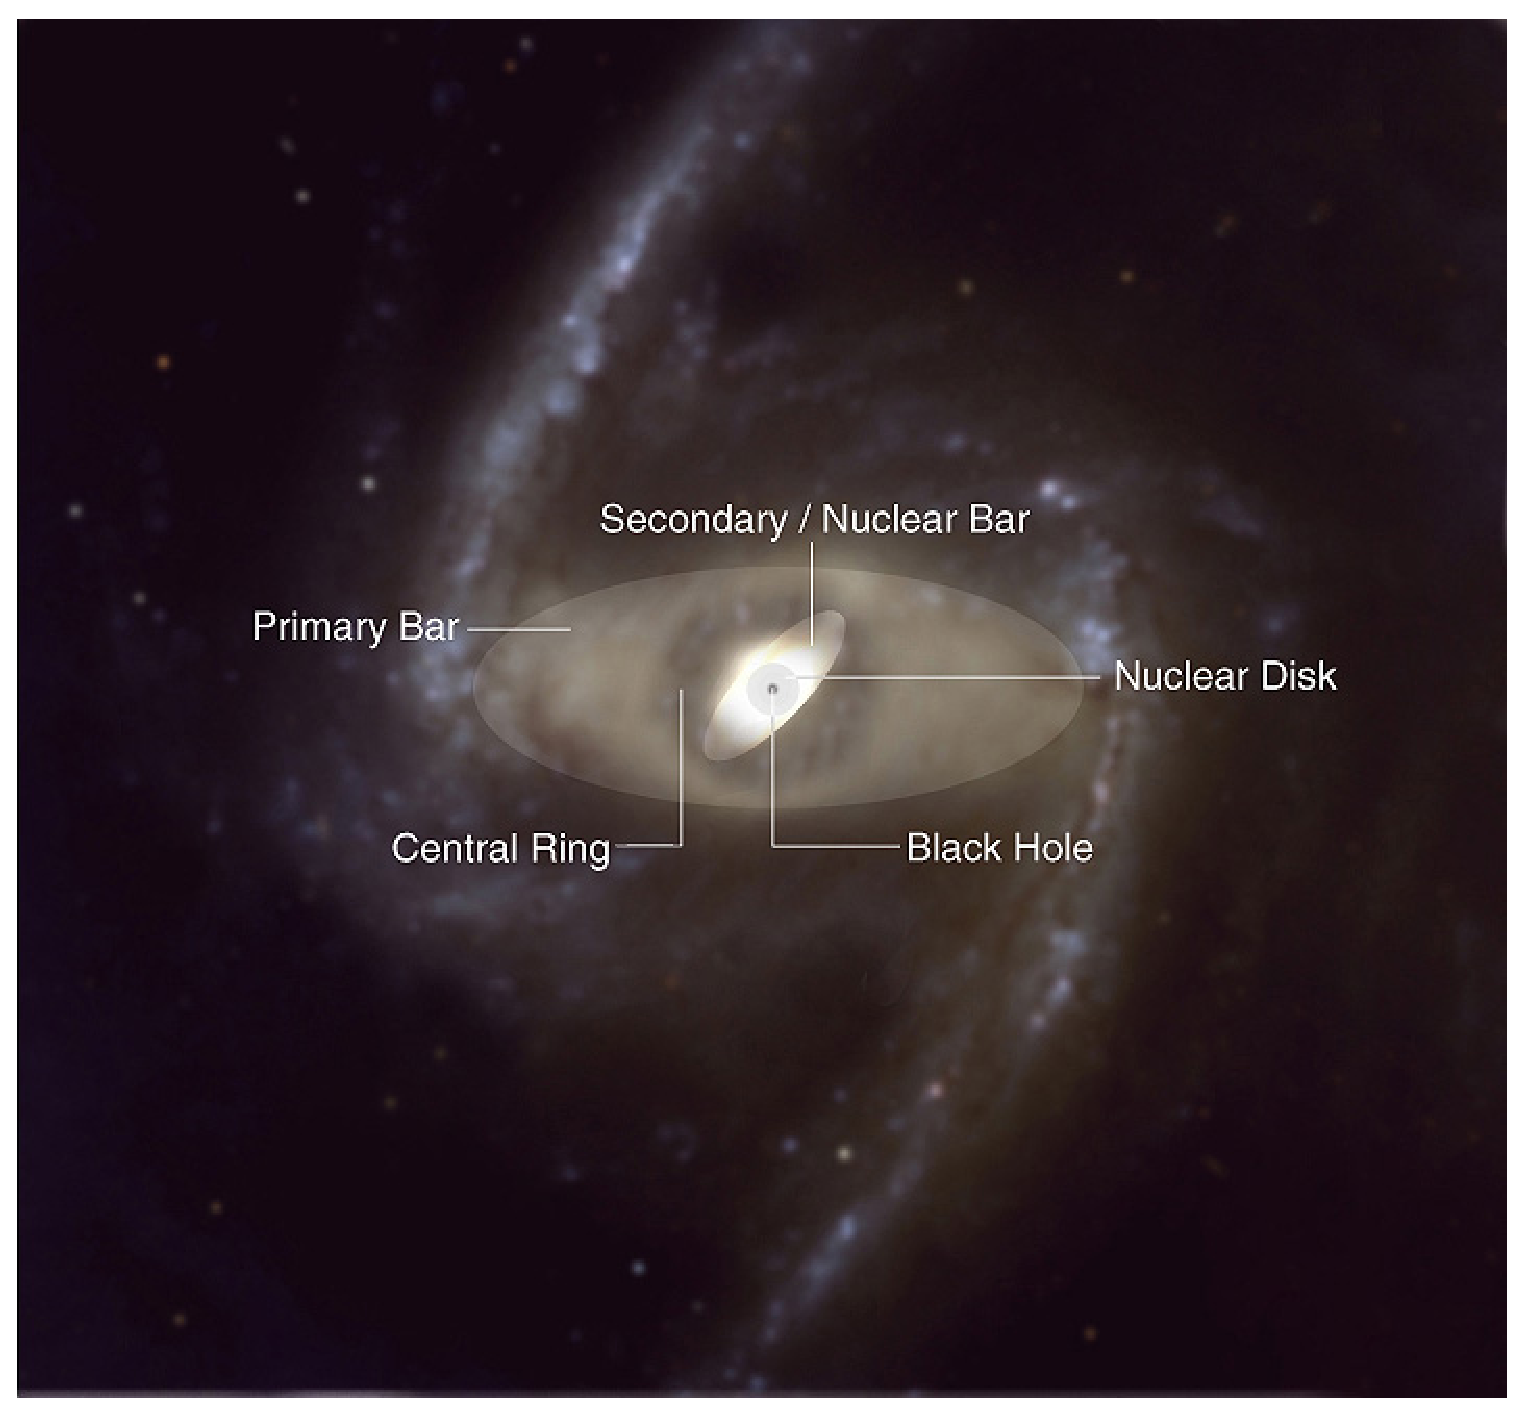
\includegraphics[width=.9\textwidth]{./eso0128d.eps}
\caption{This is a schematic drawing of the various components of a double-barred galaxy. Credit: ESO}
\label{fig:doublepic}
\end{figure}

It has been suggested that nested bars may provide a mechanism for fueling active galactic nuclei \citep{shlosman} however more recently \citep{erwin3} believe that inner bars only play a minor role in this 
activity. \citep{erwin1} compared single and double-barred galaxies and found that there was no significant difference in nuclear activity. To investigate this theory further \cite{lorenzo1} carried out a 
study of NGC 357. This study aimed to present the first detailed morphological, kinematical and stellar population analysis of the bulge, inner and outer bars of a double-barred galaxy. They concluded that
the bulge and inner bar show similar stellar population properties whilst the outer bar was less metal-rich. This result implied that, for the case of NGC 357, the outer bar was formed in a shorter timescale than
the inner structures and so disagrees with traditional idea that gas flown along the outer structure triggers star formation causing the formation of the inner structure. This was strengthened by a further study of
four double-barred galaxies by \cite{lorenzo2} where they concluded that the stellar populations of inner bars are younger and more metal-rich than the outer bars. This suggests that at present inner bars play a
moderate or even minor role in the morphological evolution of double-barred galaxies \citep{lorenzo2}.

Through the use of computer modeeling \cite{saha} showed that double bars can form without gas in a dark matter dominated halo. They produced a model where the inner bar was rotating at almost as slowly as the 
outer bar. The route to the formation of double bars maybe very different to that of a single bar.
%\citep{moiseev}, \citep{sellwood}

\subsection{N-Body Simulations and the Four-Body Problem}
Studies of three or more bodies interacting gravitationally dates back to the time of Newton. However it is only with the widespread use of computers that orbits of more than three bodies have been extensively studied. Today
N-body simulations are an essential tool in the study of solar system dynamics and galactic dynamics \citep{binney}. Celestial mechanics during the preceding centuries has mainly focussed on the three body problem
due to the complexities involved in adding more bodies. It is estimated that within the Milky Way approximately two thirds of all stars exist in binary systems and a further one fifth of these are in triple systems whilst a
further fifth still exist in systems with more than three bodies \citep{steves}. \cite{steves} estimate that $\approx2\times10^9$ quadruple systems exist in the Milky Way galaxy. They found that quadruple systems exist in two
forms: a double binary or linear.
\newline
The classical equations of motion for an N-body problem are:
\begin{equation}
m_i\mathbf{\ddot{r}}=\sum_{i\neq{j}}\frac{{m_i}{m_j}}{r^3_{ij}}\mathbf{r_{ij}}
\qquad
i=1,2,3...
\end{equation}
where $\mathbf{r_i}=\left(x_i,y_i\right)$ and $\mathbf{r_{ij}}=\mathbf{r_j}-\mathbf{r_i}$. 
The units have been selected so that the gravitational constant (G) is equal to one. In simulations it is natural to choose units where G = 1 and the units of length nand mass are conventionally chosen
so that the total mass of the system is M = 1 \citep{heggie}.

The four body problem, specifically, has been studied extensively by \cite{steves}. Here they model four equal mass bodies orbiting in circular coplanar orbits. This model they term the Caledonian problem, because
their research is being carried out at Glasgow Caledonian University.
Approximately a century ago the Copenhagen problem was studied extensively in Copenhagen which consisted of a three body problem: two equal mass bodies and an infinitesimally small test particle. \cite{szell} also
studied the Caledonian problem and found that the stability of the system is dependent upon a constant termed the Szebehely constant. The Caledonian Symmetric Double Binary Problem (CSDBP) is relevant in 
studying the stability and evolution of symmetric quadruple stellar clusters and exoplanetary systems of two planets orbiting a binary pair of stars \citep{alvarez}.

Methods for the study of N-body simulations have changed considerably since the advent of computers. In a study of N-body simulations \cite{trenti} mentions a pioneering attempt by Holmberg in 1941 which used 
light bulbs and galvanometers to track the evolution of 37 particles. However it wasn't until the early seventies and the advent of computers that this field really got started. 
Nowadays simulations can up to a million particles \citep{heggie} which is of particular relevance to the study of globular
clusters. I refer the reader to \cite{aarseth} for much more detailed explanation of the field of N-body simulations.
 %\citep{collins}, \citep{moulton}

\subsection{Orbits, Loops, Resonances and Double-Barred Galaxy Simulations}
Double-barred galaxy simulations and models have taken many forms. \cite{du1} explored the formation and evolution of double-barred galaxies (which is not very well understood) by showing that a dynamically
cool inner disk embedded in a hotter outer disk can generate a secondary bar while the outer disk forms a large-scale primary bar. \cite{macie8} used hydrodynamical simulations to study gas inflow in barred galaxies
and the effect this has on secondary bars. They concluded that the secondary bar can prevent, rather than enhance, the inflow. More recently, \cite{debattista} used collisionless N-body simulations to show
that inner bars can form spontaneously without requiring gas. They also found that secondary bars rotate faster that primary bars and that the secondary bars pulsate. This is considered further in the Discussion.

In an attempt to explain the dynamics of the orbits of nested bars \cite{macie7} introduced the concept of `loops'. They wanted to investigate how two independently rotating bars can maintain
themselves as gravitating systems. A gravitational potential consisting of two concentric bisymmetric bars that are independently rotating is not stationary in any reference frame \cite{macie7}. In the potential
of a single bar particles would stay on a stable closed periodic orbit but with nested bars orbits will not be closed because the particles would be experience two separate forces. The `loop' therefore was
introduced as an extension of the concept of orbit. Particles in a `loop' would return to their original positions every time the bars come back to the same relative orientation \citep{macie7}. This lead to
the conclusion that loops supporting the inner bar are thicker with parallel bars and thinner with perpendicular bars \citep{macie3}. This also suggets that the two bars do not rotate through each other as rigid bodies
but the inner bar should pulsate and that the bars should spend more time nearly orthognal\citep{macie3}. These predictions were confirmed by \citep{debattista} and \citep{shen1}. 
This was further confirmed by \cite{macie5} who found
that the inner bar should end well within its corotation radius and that the inner bar extends further out for lower pattern speeds than higher ones; the inner bar pulsates; and that the angular velocity of the inner
bar is not uniform and that faster inner bars rotate more coherently.

\cite{wozniak} also carried out double-barred galaxy simulations and achieved long-lived inner bars lasting for up to 7 Gyr. These were N-body/hydrodynamical simulations. They found that the two bar lengths, ratio of
pattern speeds, as well as the age of the inner stellar bar populations in the simulations matched well with observations. They concluded that because, unlike previous simulations, there was no overlap between primary bar 
inner Lindblad resonance (ILR) and the inner bar corotation (CR) or any kind of resonance overlap, then some other kind of mechanism must feed the central waves \citep{wozniak}. It is suggested that star 
formation may be responsible for bringing energy into the inner bar.

\cite{garzon} studied the dynamical evolution of two isolated bars, within the same galaxy, under their mutual gravitational interaction. They considered two cases purely analytically: rotation of rigid bodies and
rotation of deformable rotation. They found that the bars oscillate in size according to the relative angle between the bars. This is broadly in agreement with \citep{debattista}.
What follows is an attempt to verify the calculations in \citep{garzon} but using a simpler model of a double-barred galaxy using a double binary.
 %\citep{du2}, \citep{macie1}, \citep{macie2},  \citep{macie4}
 %\citep{malhotra}, \citep{manos}, \citep{shen2}

\section{Methods}
Fortran 90 was selected as the language of choice in order to avoid the fixed line limitations of Fortran 77.
The model was created using OdeInt from Numerical Recipes. I first converted OdeInt to Fortran 90 for this purpose.
For a four body problem 
this equation results in the following:
\begin{equation}
\ddot{\mathbf{r_1}}=\frac{m_2\mathbf{r}_{12}}{r^3_{12}}+\frac{m_3\mathbf{r}_{13}}{r^3_{13}}+\frac{m_4\mathbf{r}_{14}}{r^3_{14}}
\end{equation}
\begin{equation}
\ddot{\mathbf{r_2}}=\frac{m_1\mathbf{r}_{21}}{r^3_{21}}+\frac{m_3\mathbf{r}_{23}}{r^3_{23}}+\frac{m_4\mathbf{r}_{24}}{r^3_{24}}
\end{equation}
\begin{equation}
\ddot{\mathbf{r_3}}=\frac{m_1\mathbf{r}_{31}}{r^3_{31}}+\frac{m_2\mathbf{r}_{32}}{r^3_{32}}+\frac{m_4\mathbf{r}_{34}}{r^3_{34}}
\end{equation}
\begin{equation}
\ddot{\mathbf{r_4}}=\frac{m_1\mathbf{r}_{41}}{r^3_{41}}+\frac{m_2\mathbf{r}_{42}}{r^3_{42}}+\frac{m_3\mathbf{r}_{43}}{r^3_{43}}
\end{equation}
The above equations were encoded into Fortran. A full code listing is supplied in a separate file.
\subsection{Initial Conditions}
As a starting point both the outer binary and inner binary were placed in circular orbits and tested separately and then combined to ensure a stable
starting point. The inner binary had initially a neglible mass.
The outer binary initial conditions were:
\begin{lstlisting}
m1=.5, m2=.5, x1=-.5, x2=.5, y1=0, y2=0,
vx1=0, vx2=0, vy1=-.5, vy2=.5
\end{lstlisting}
and for the inner binary:
\begin{lstlisting}
m3=.001, m4=.001, x3=-.001, x4=.001, y3=0, y4=0, 
vx3=0, vx4=0, vy3=-.5, vy4=.5
\end{lstlisting}
Plots of the two initial binaries are shown in Fig. \ref{fig:outerbinary} and 
\ref{fig:innerbinary}. The scale of the inner binary is so small that it is difficult
to see in GnuPlot.
\begin{figure}[H]
\centering
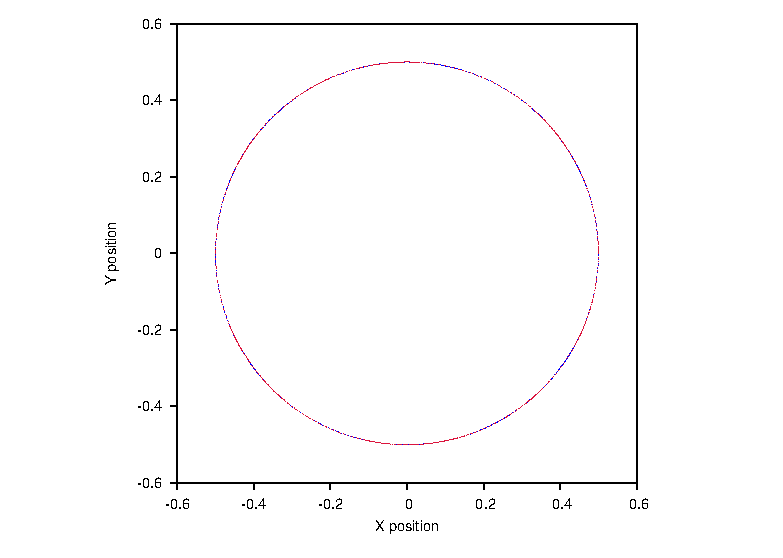
\includegraphics[width=.9\textwidth]{./2016results/outerbinary/Orbit.eps}
\caption{Outer Binary}
\label{fig:outerbinary}
\end{figure}
\begin{figure}[H]
\centering
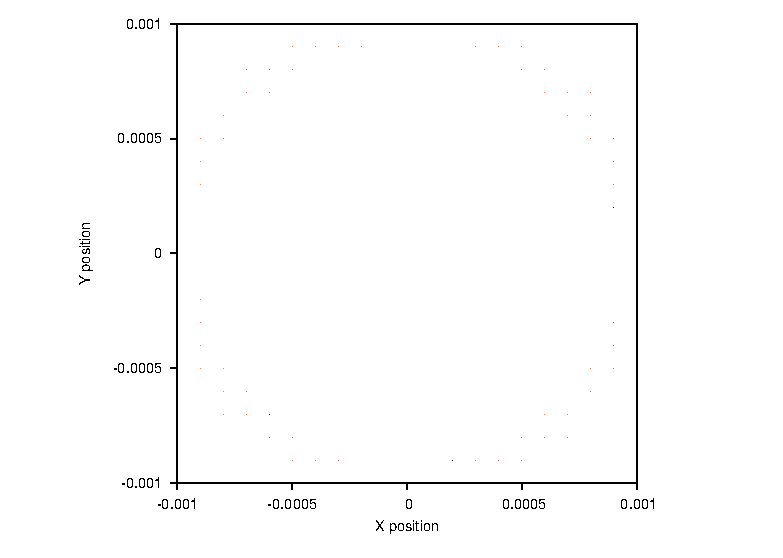
\includegraphics[width=.9\textwidth]{./2016results/innerbinary/Orbit.eps}
\caption{Inner Binary}
\label{fig:innerbinary}
\end{figure}
I then proceeded to perturb the system by gradually increasing the mass of the inner binary. As the system became unstable I componensated for
the increasing mass of the inner binary by increasing the velocity of the outer binary and also decreasing the velocity and increasing the binary 
separation of the inner binary. In many of the configurations the systems were inherently unstable and produced collisions with some 
or all of the bodies being ejected from the system. These were rejected and only 'stable' configurations were considered.
Table \ref{tab:variables} shows the perturbations made to the system - only the variables in this table changed and all the other initial
conditions remained the same.
\begin{table}[ht!]
  \centering
  \caption{Configurations}
  \label{tab:variables}
  \begin{tabular}{ccccccccc}
   Config. & m3 & m4 & vy1 & vy2 & x3 & x4 & vy3 & vy4\\
    \hline
   1 & .001 & .001 & -.5 & .5 & -.001 & .001 & -.5 & .5\\
   2 & .002 & .002 & -.5 & .5 & -.001 & .001 & -.5 & .5\\
   3 & .003 & .003 & -.5 & .5 & -.001 & .001 & -.5 & .5\\
   4 & .004 & .004 & -.5 & .5 & -.004 & .004 & -.5 & .5\\
   5 & .004 & .004 & -.55 & .55 & -.004 & .004 & -.5 & .5\\
   6 & .004 & .004 & -.57 & .57 & -.004 & .004 & -.5 & .5\\
   7 & .005 & .005 & -.58 & .58 & -.005 & .005 & -.3 & .3\\
   8 & .005 & .005 & -.58 & .58 & -.005 & .005 & -.4 & .4\\
   9 & .005 & .005 & -.58 & .58 & -.005 & .005 & -.35 & .35\\
   10 & .006 & .006 & -.6 & .6 & -.006 & .006 & -.3 & .3\\
   11 & .025 & .025 & -.65 & .65 & -.02 & .02 & -.5 & .5\\
   12 & .025 & .025 & -.7 & .7 & -.025 & .025 & -.5 & .5\\
   13 & .03 & .03 & -.7 & .7 & -.03 & .03 &-.5 & .5\\
   14 & .035 & .035 & -.75 & .75 & -.04 & .04 &-.4 & .4\\
   15 & .04 & .04 & -.75 & .75 & -.045 & .045 &-.4 & .4\\
   16 & .05 & .05 & -.75 & .75 & -.045 & .045 &-.4 & .4\\
   17 & .05 & .05 & -.75 & .75 & -.05 & .05 &-.35 & .35\\
   18 & .05 & .05 & -.75 & .75 & -.05 & .05 &-.3 & .3\\
   19 & .06 & .06 & -.8 & .8 & -.06 & .06 &-.25 & .25\\
   20 & .08 & .08 & -.9 & .9 & -.08 & .08 &-.15 & .15\\
   21 & .09 & .09 & -.95 & .95 & -.09 & .09 &-.1 & .1\\
   22 & .1 & .1 & -1 & 1 & -.1 & .1 & -.05 & .05\\
   23 & .1 & .1 & -1 & 1 & -.1 & .1 & -.04 & .04\\
   24 & .1 & .1 & -1 & 1 & -.1 & .1 & -.03 & .03\\
   25 & .1 & .1 & -1 & 1 & -.1 & .1 & -.02 & .02\\
   26 & .12 & .12 & -1.05 & 1.05 & -.11 & .11 & -.015 & .015\\
   27 & .12 & .12 & -1.1 & 1.1 & -.11 & .11 & -.015 & .015\\
   28 & .12 & .12 & -1.1 & 1.1 & -.115 & .115 & -.015 & .015\\
   29 & .12 & .12 & -1.1 & 1.1 & -.12 & .12 & -.015 & .015\\
   30 & .1 & .1 & -1 & 1 & -.1 & .1 & -.1 & .1\\
   31 & .1 & .1 & -1 & 1 & -.102 & .102 & -.1 & .1\\
   31 & .1 & .1 & -1 & 1 & -.1021 & .1021 & -.1 & .1\\
  \end{tabular}
\end{table}

\subsection{Compilers}
As I had converted OdeInt into Fortran 90 I wanted to make sure I hadn't introduced any errors. I therefore compared the output of the Numerical Recipes
version of OdeInt with mine. I was compiling with GFortran and the Fortran 77 version was compiled with g77. They were different! So naturally concerned 
I then compiled the Fortran 77 version with GFortran. The results were identical to mine, which satisified me that I hadn't introduced any errors.

\section{Results}
As can be seen from Fig. \ref{fig:config1} even a neglible mass inner binary causes the outer binary to begin to separate and become less tightly bound.
Figures Fig. \ref{fig:config1} to \ref{fig:config18i} show plots of the double binary using the parameters given in Table \ref{tab:variables}.
In many cases the inner binary is only visible as a point at the centre of the outer binary.
As the mass of the inner binary increased the system became increasingly unstablle and the effect on the outer binary became more pronounced.
Even the 'stable' configurations listed in Table \ref{tab:variables} hold for only a few orbits.
I was unable to recreate a stable system for a mass $>.08$ for the inner bar.
The plots below reveal that increasing the mass of the inner binary causes the outer binary to separate and
form wider orbits.

\begin{figure}[H]
\centering
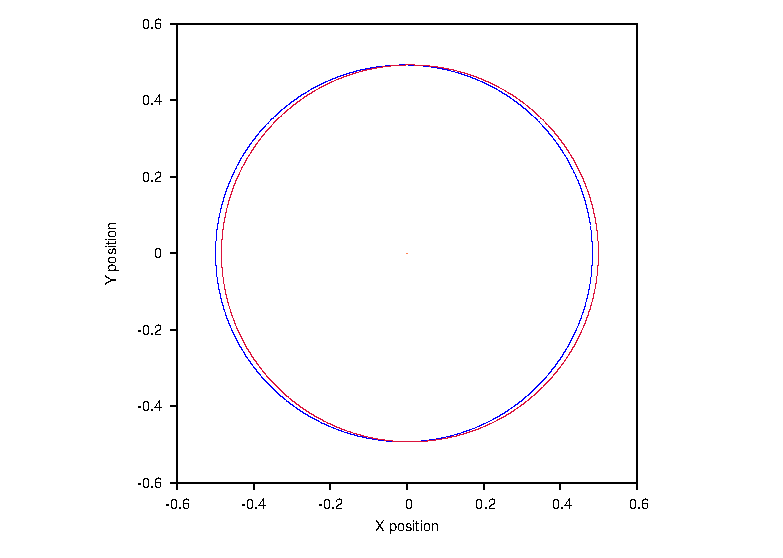
\includegraphics[width=.9\textwidth]{./2016results/stablebase/Orbit.eps}
\caption{Configuration 1}
\label{fig:config1}
\end{figure}

\begin{figure}[H]
\centering
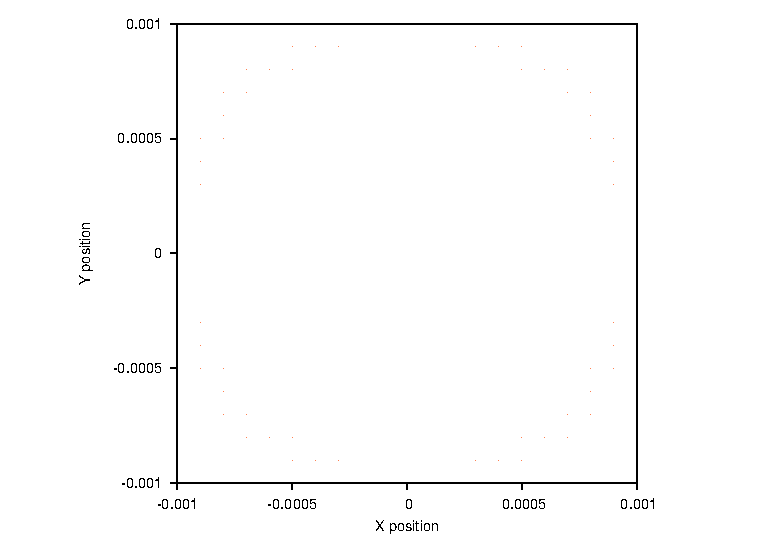
\includegraphics[width=.9\textwidth]{./2016results/stablebase/Inner.eps}
\caption{Configuration 1 - Inner Bar}
\label{fig:config1i}
\end{figure}

\begin{figure}[H]
\centering
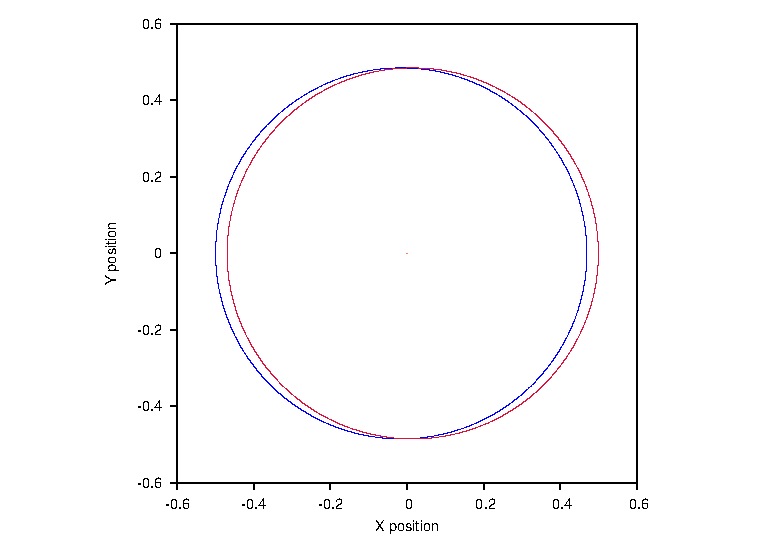
\includegraphics[width=.9\textwidth]{./2016results/002-5-001/Orbit.eps}
\caption{Configuration 2}
\label{fig:config2}
\end{figure}

\begin{figure}[H]
\centering
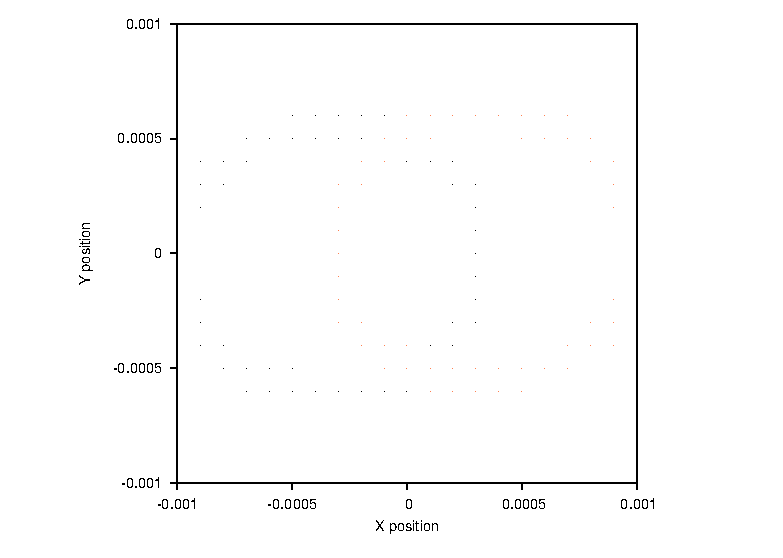
\includegraphics[width=.9\textwidth]{./2016results/002-5-001/Inner.eps}
\caption{Configuration 2 - Inner Bar}
\label{fig:config2i}
\end{figure}

\begin{figure}[H]
\centering
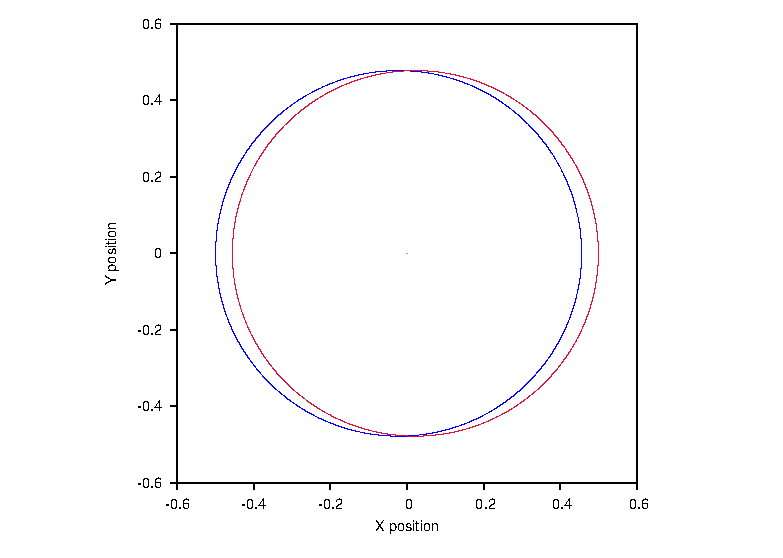
\includegraphics[width=.9\textwidth]{./2016results/003-5-001/Orbit.eps}
\caption{Configuration 3}
\label{fig:config3}
\end{figure}
\begin{figure}[H]
\centering
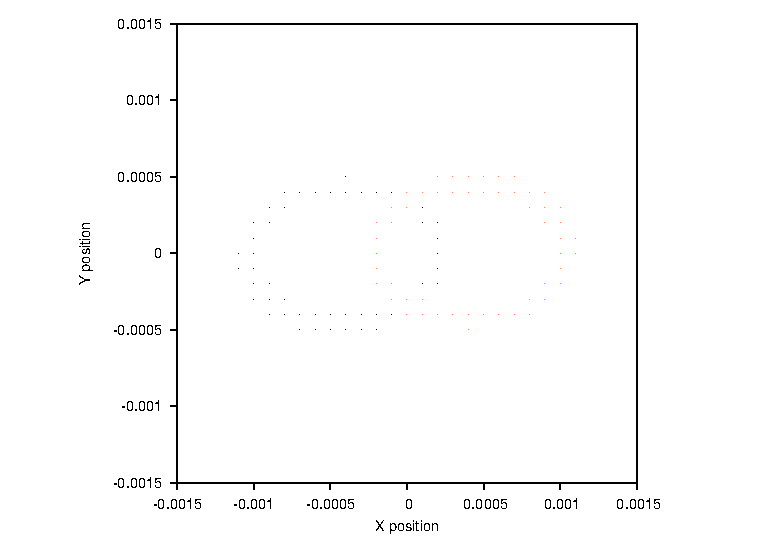
\includegraphics[width=.9\textwidth]{./2016results/003-5-001/Inner.eps}
\caption{Configuration 3 - Inner Bar}
\label{fig:config3i}
\end{figure}

\begin{figure}[H]
\centering
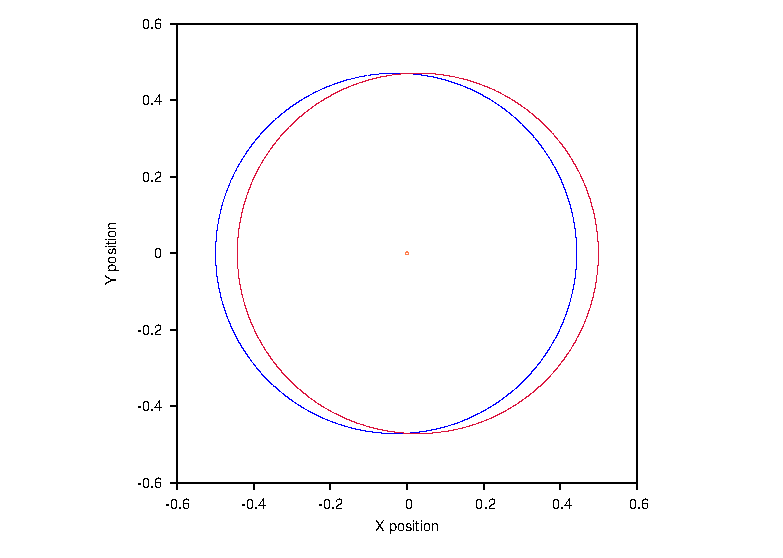
\includegraphics[width=0.9\textwidth]{./2016results/004-5-004/Orbit.eps}
\caption{Configuration 4}
\label{fig:config4}
\end{figure}
\begin{figure}[H]
\centering
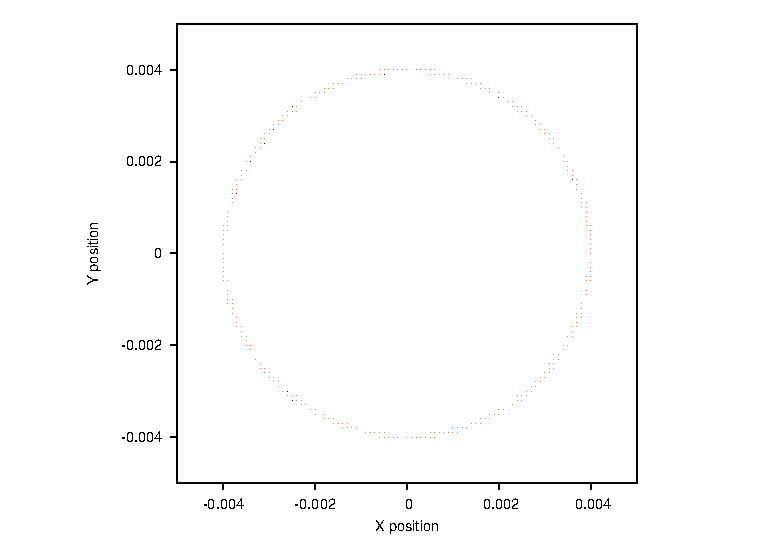
\includegraphics[width=0.9\textwidth]{./2016results/004-5-004/Inner.eps}
\caption{Configuration 4 - Inner Bar}
\label{fig:config4i}
\end{figure}
l
\begin{figure}[H]
\centering
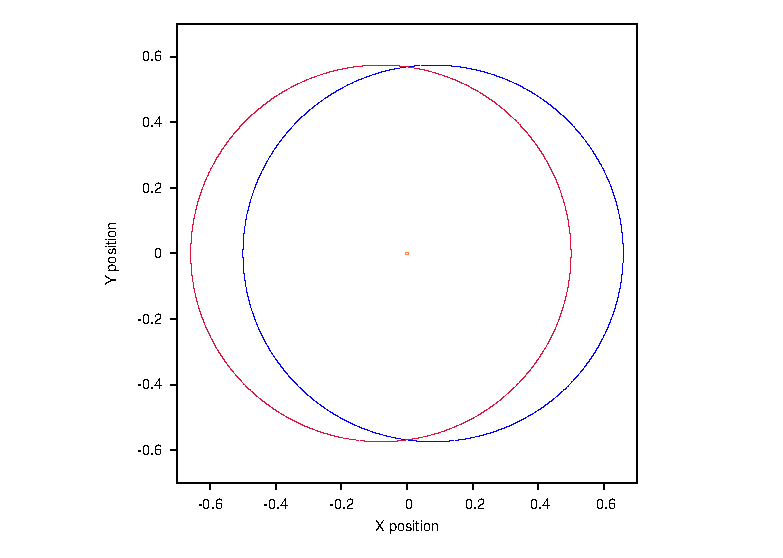
\includegraphics[width=0.9\textwidth]{./2016results/004-55-004/Orbit.eps}
\caption{Configuration 5}
\label{fig:config5}
\end{figure}
\begin{figure}[H]
\centering
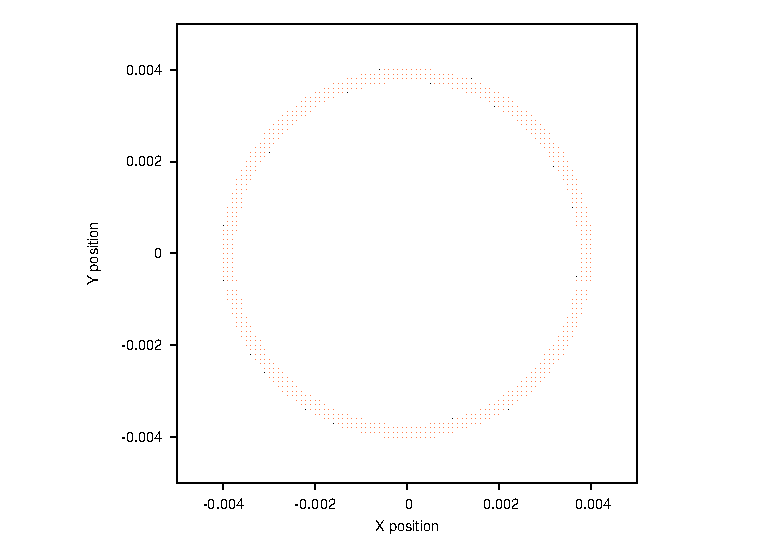
\includegraphics[width=0.9\textwidth]{./2016results/004-55-004/Inner.eps}
\caption{Configuration 5 - Inner Bar}
\label{fig:config5i}
\end{figure}

\begin{figure}[H]
\centering
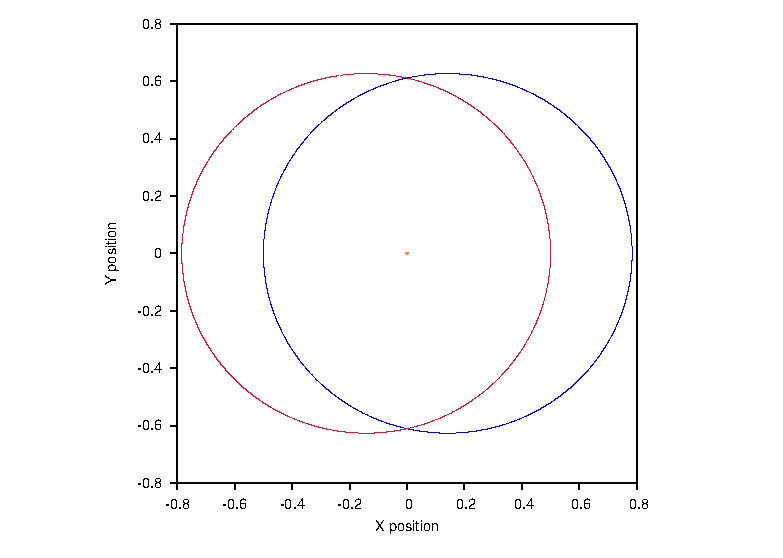
\includegraphics[width=0.9\textwidth]{./2016results/004-57-004/Orbit.eps}
\caption{Configuration 6}
\label{fig:config6}
\end{figure}
\begin{figure}[H]
\centering
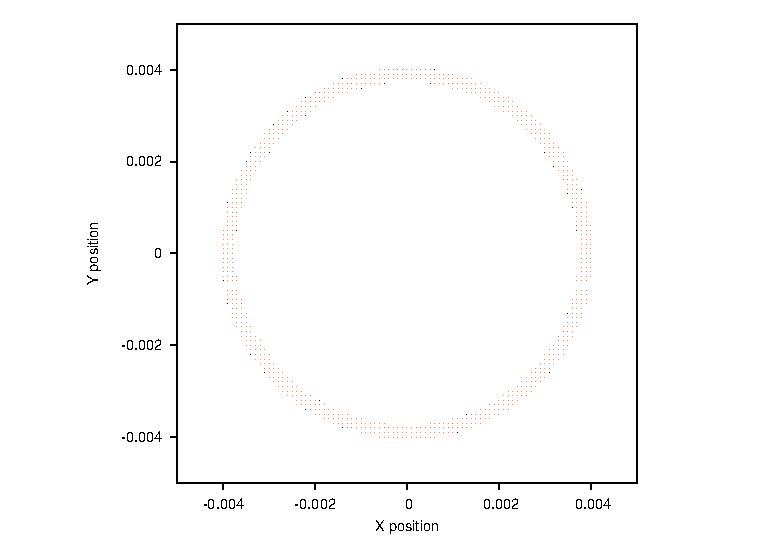
\includegraphics[width=0.9\textwidth]{./2016results/004-57-004/Inner.eps}
\caption{Configuration 6 - Inner Bar}
\label{fig:config6i}
\end{figure}

\begin{figure}[H]
\centering
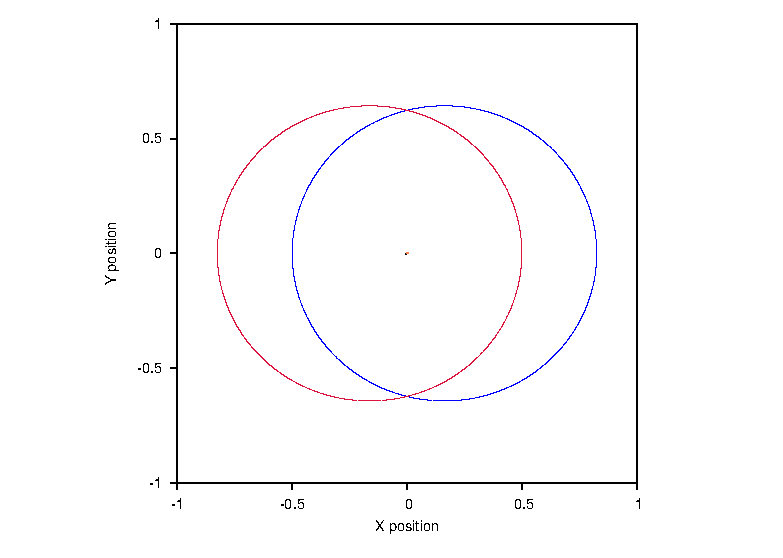
\includegraphics[width=0.9\textwidth]{./2016results/005-58-005-3/Orbit.eps}
\caption{Configuration 7}
\label{fig:config7}
\end{figure}
\begin{figure}[H]
\centering
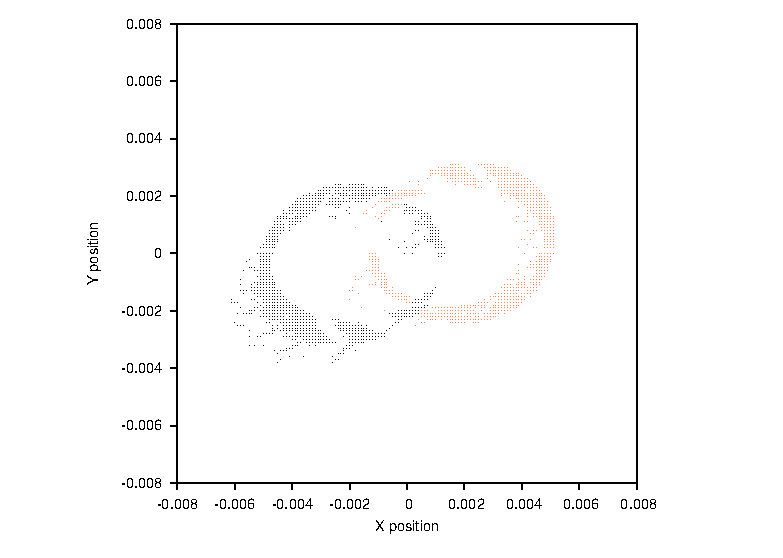
\includegraphics[width=0.9\textwidth]{./2016results/005-58-005-3/Inner.eps}
\caption{Configuration 7 - Inner Bar}
\label{fig:config7i}
\end{figure}

\begin{figure}[H]
\centering
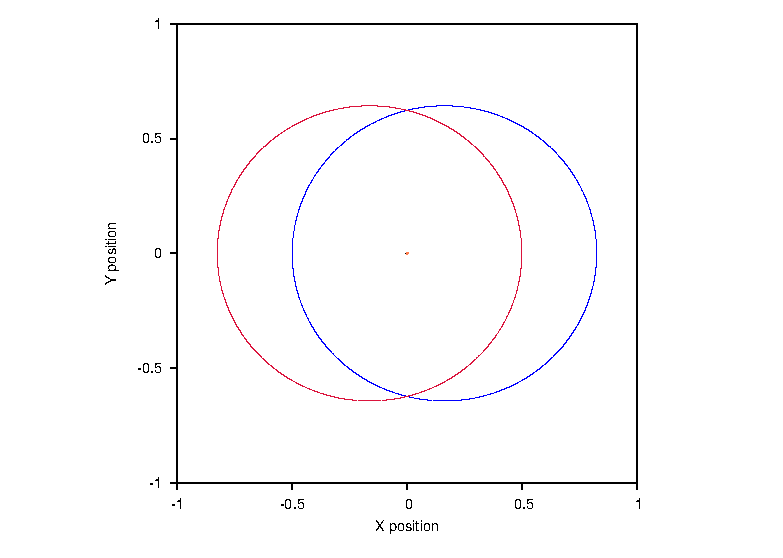
\includegraphics[width=0.9\textwidth]{./2016results/005-58-005-4/Orbit.eps}
\caption{Configuration 8}
\label{fig:config8}
\end{figure}
\begin{figure}[H]
\centering
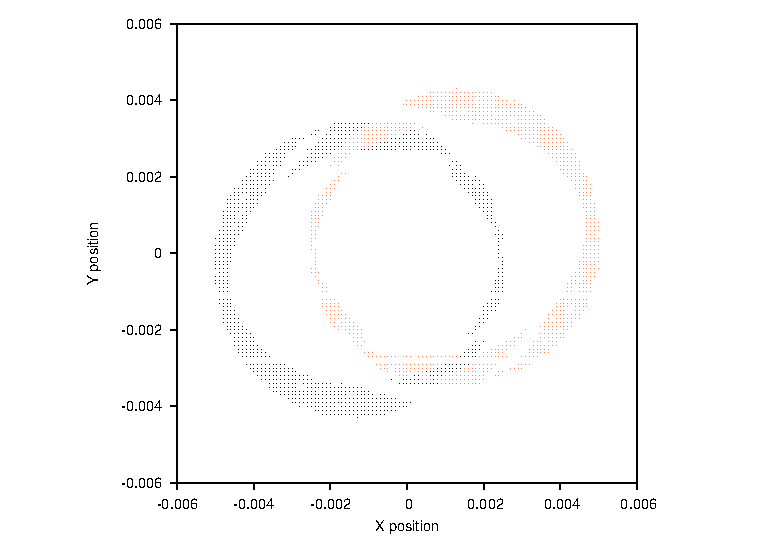
\includegraphics[width=0.9\textwidth]{./2016results/005-58-005-4/Inner.eps}
\caption{Configuration 8 - Inner Bar}
\label{fig:config8i}
\end{figure}

\begin{figure}[H]
\centering
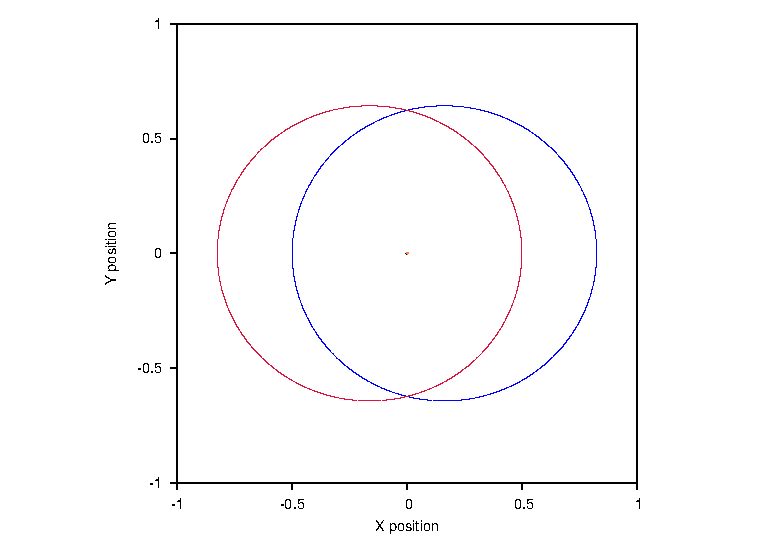
\includegraphics[width=0.9\textwidth]{./2016results/005-58-005-35/Orbit.eps}
\caption{Configuration 9}
\label{fig:config9}
\end{figure}
\begin{figure}[H]
\centering
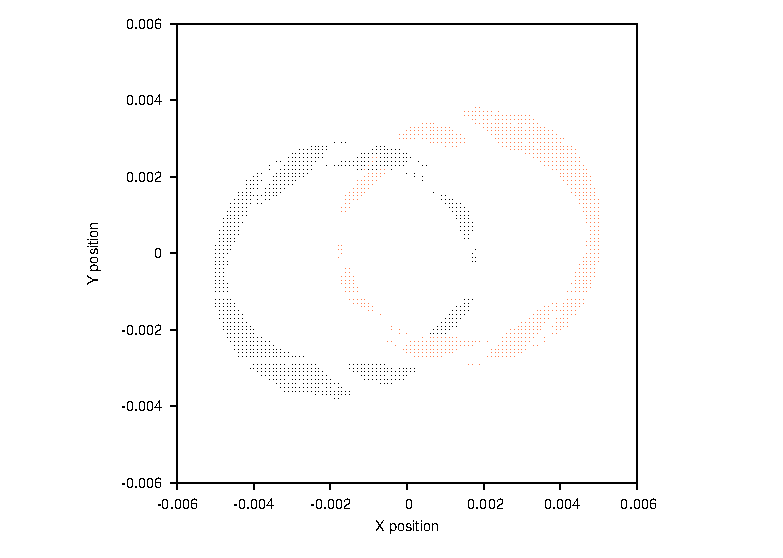
\includegraphics[width=0.9\textwidth]{./2016results/005-58-005-35/Inner.eps}
\caption{Configuration 9 - Inner Bar}
\label{fig:config9i}
\end{figure}

\begin{figure}[H]
\centering
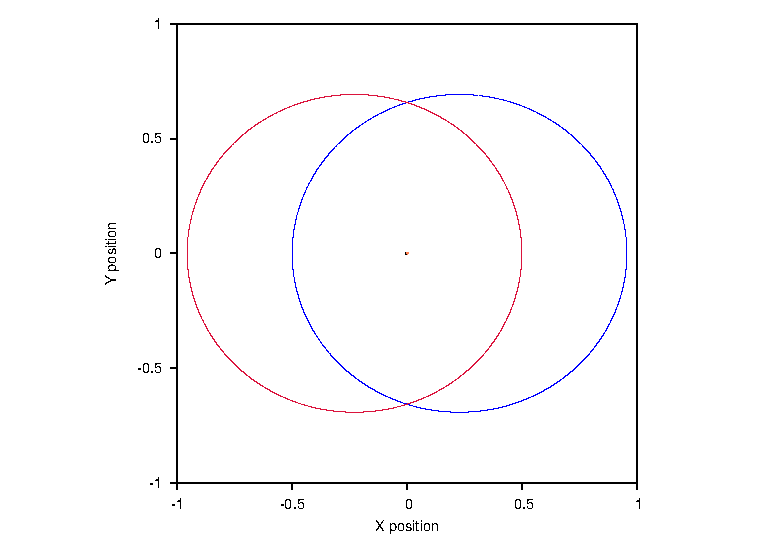
\includegraphics[width=0.9\textwidth]{./2016results/006-6-006-3/Orbit.eps}
\caption{Configuration 10}
\label{fig:config10}
\end{figure}
\begin{figure}[H]
\centering
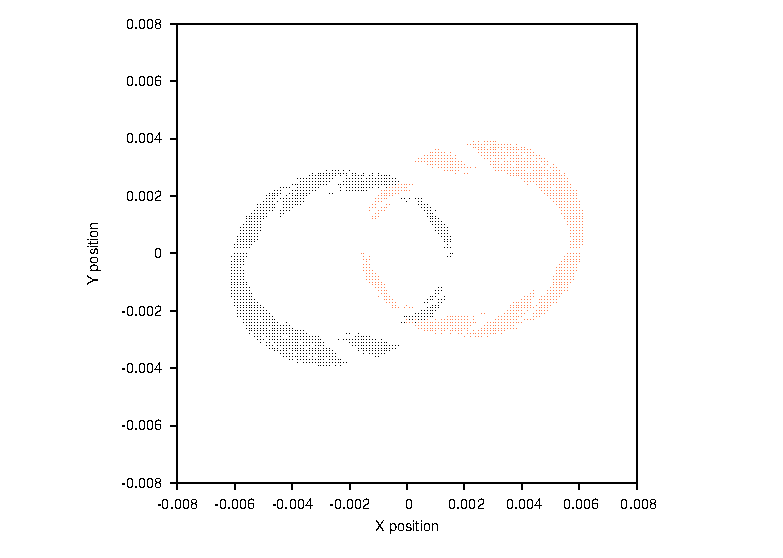
\includegraphics[width=0.9\textwidth]{./2016results/006-6-006-3/Inner.eps}
\caption{Configuration 10 - Inner Bar}
\label{fig:config10i}
\end{figure}

\begin{figure}[H]
\centering
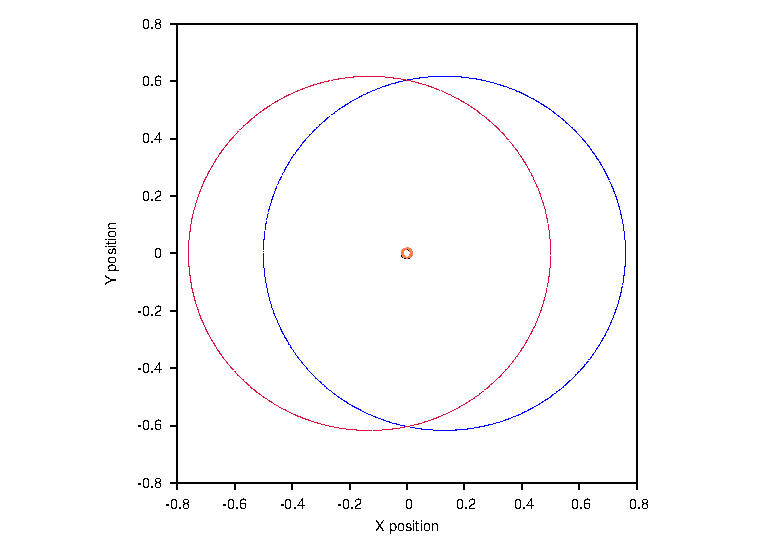
\includegraphics[width=0.9\textwidth]{./2016results/025-65-02/Orbit.eps}
\caption{Configuration 11}
\label{fig:config11}
\end{figure}
\begin{figure}[H]
\centering
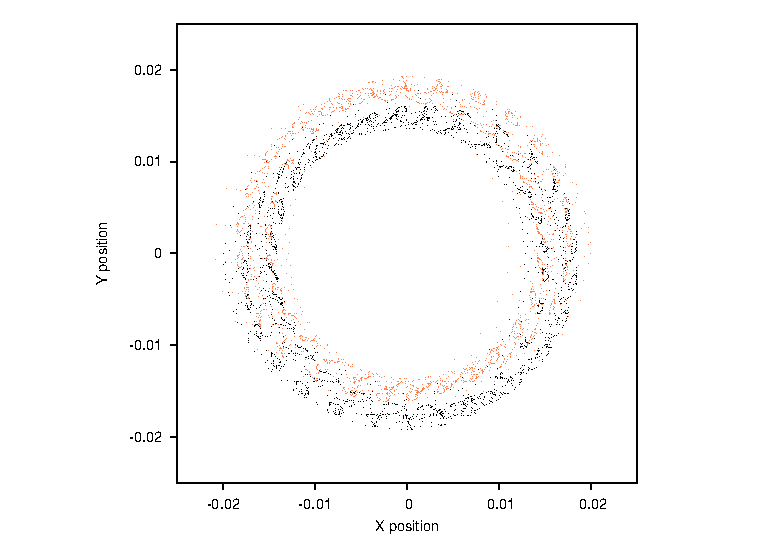
\includegraphics[width=0.9\textwidth]{./2016results/025-65-02/Inner.eps}
\caption{Configuration 11 - Inner Bar}
\label{fig:config11i}
\end{figure}

\begin{figure}[H]
\centering
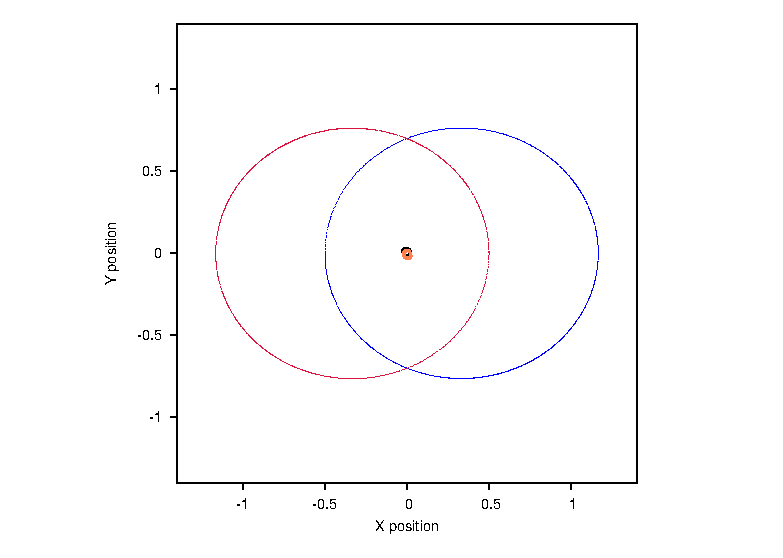
\includegraphics[width=0.9\textwidth]{./2017results/025-7-025-5/Orbit.eps}
\caption{Configuration 12}
\label{fig:config12}
\end{figure}
\begin{figure}[H]
\centering
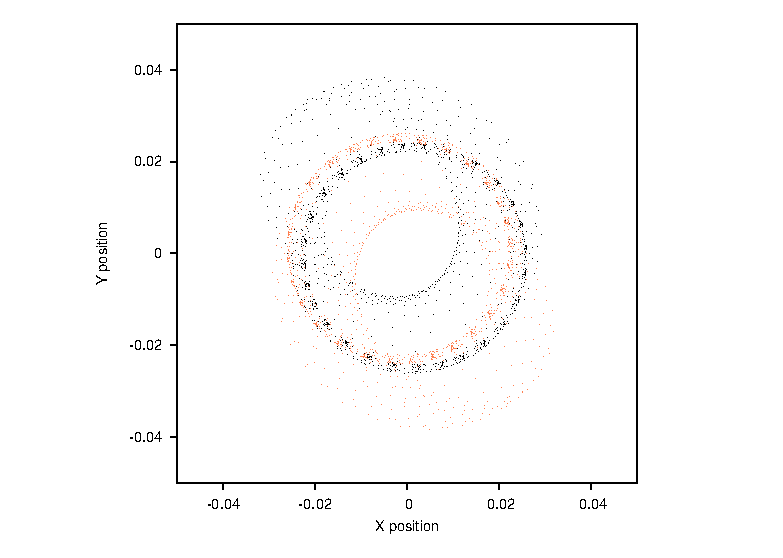
\includegraphics[width=0.9\textwidth]{./2017results/025-7-025-5/Inner.eps}
\caption{Configuration 12 - Inner Bar}
\label{fig:config12i}
\end{figure}

\begin{figure}[H]
\centering
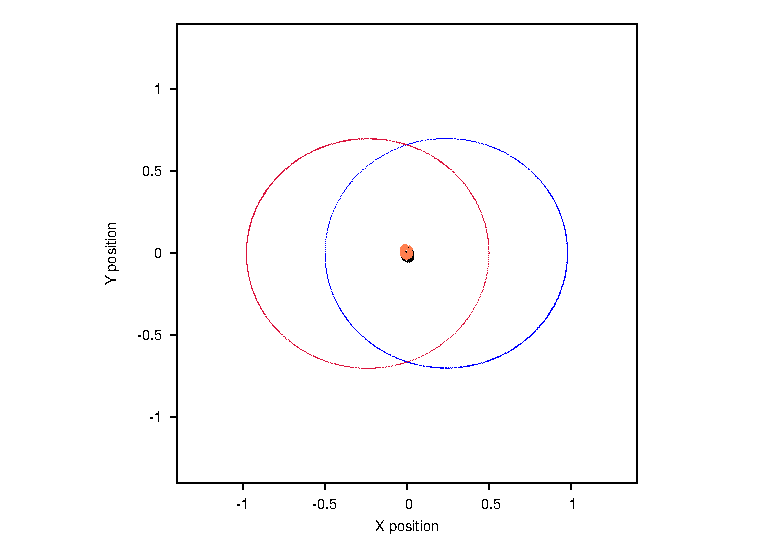
\includegraphics[width=0.9\textwidth]{./2017results/03-7-03-5/Orbit.eps}
\caption{Configuration 13}
\label{fig:config13}
\end{figure}
\begin{figure}[H]
\centering
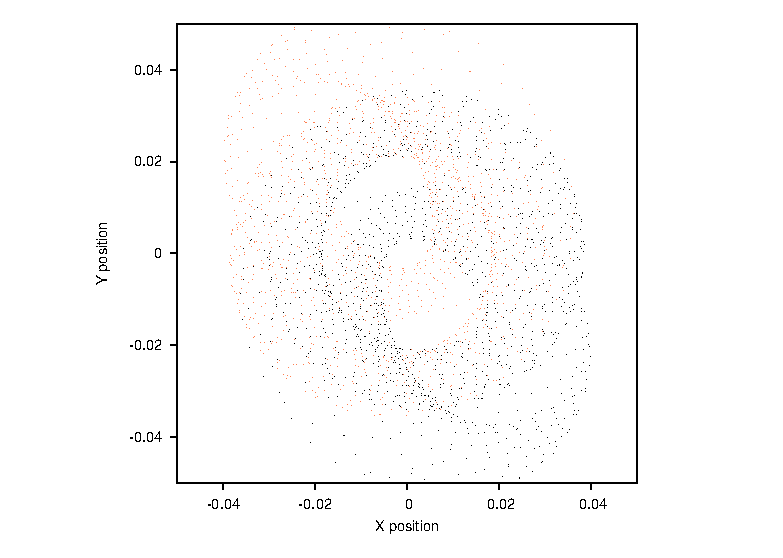
\includegraphics[width=0.9\textwidth]{./2017results/03-7-03-5/Inner.eps}
\caption{Configuration 13 - Inner Bar}
\label{fig:config13i}
\end{figure}

\begin{figure}[H]
\centering
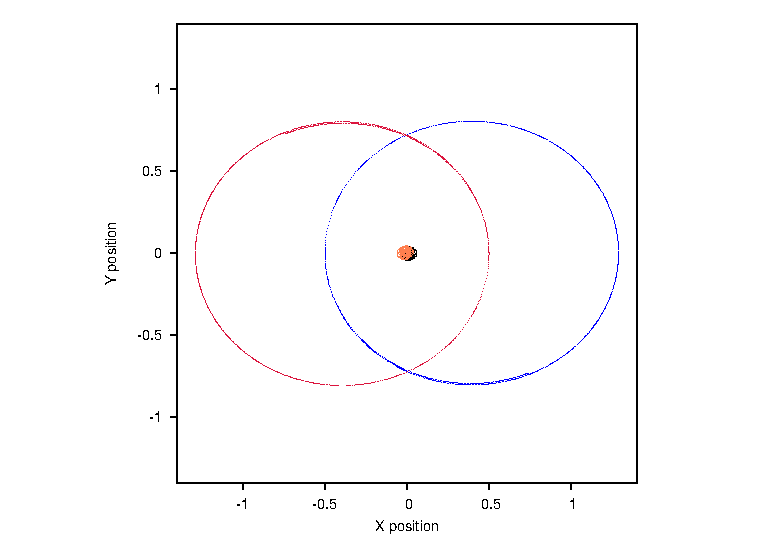
\includegraphics[width=0.9\textwidth]{./2017results/035-75-04-4/Orbit.eps}
\caption{Configuration 14}
\label{fig:config14}
\end{figure}
\begin{figure}[H]
\centering
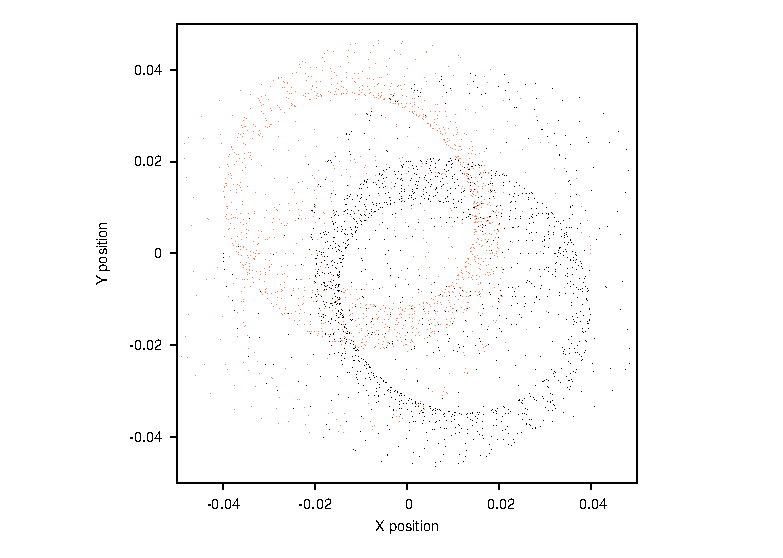
\includegraphics[width=0.9\textwidth]{./2017results/035-75-04-4/Inner.eps}
\caption{Configuration 14 - Inner Bar}
\label{fig:config14i}
\end{figure}

\begin{figure}[H]
\centering
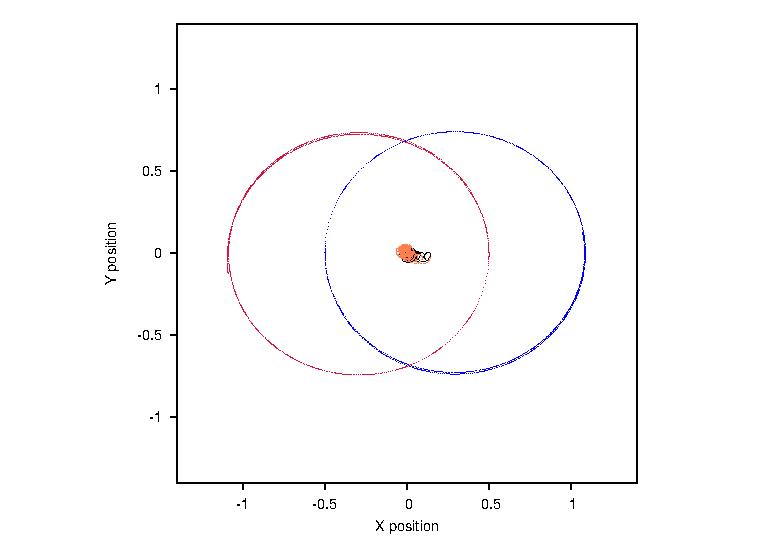
\includegraphics[width=0.9\textwidth]{./2017results/04-75-045-4/Orbit.eps}
\caption{Configuration 15}
\label{fig:config15}
\end{figure}
\begin{figure}[H]
\centering
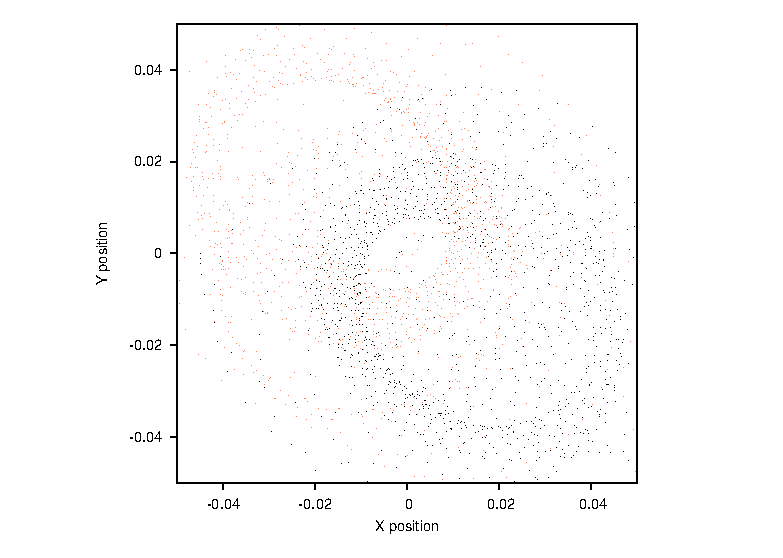
\includegraphics[width=0.9\textwidth]{./2017results/04-75-045-4/Inner.eps}
\caption{Configuration 15 - Inner Bar}
\label{fig:config15i}
\end{figure}

\begin{figure}[H]
\centering
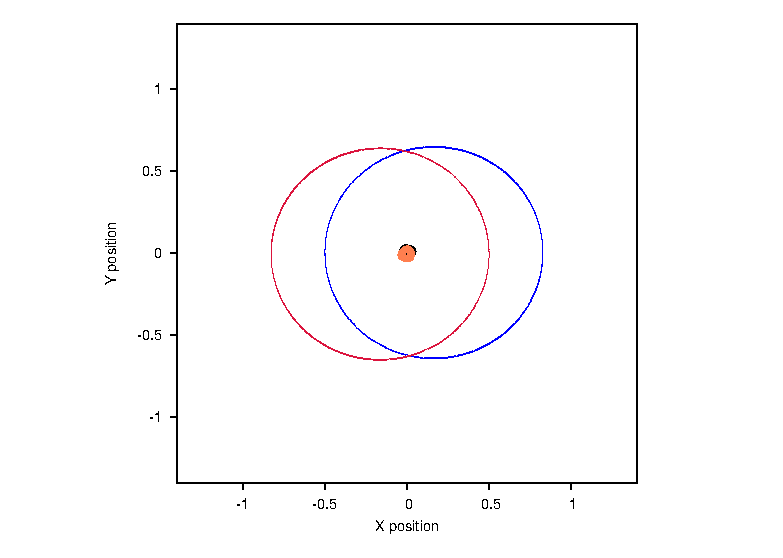
\includegraphics[width=0.9\textwidth]{./2017results/05-75-045-4/Orbit.eps}
\caption{Configuration 16}
\label{fig:config16}
\end{figure}
\begin{figure}[H]
\centering
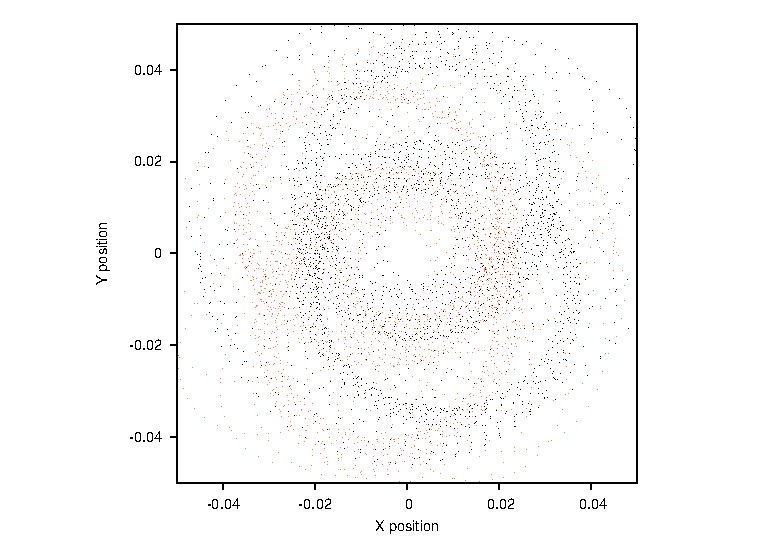
\includegraphics[width=0.9\textwidth]{./2017results/05-75-045-4/Inner.eps}
\caption{Configuration 16 - Inner Bar}
\label{fig:config16i}
\end{figure}

\begin{figure}[H]
\centering
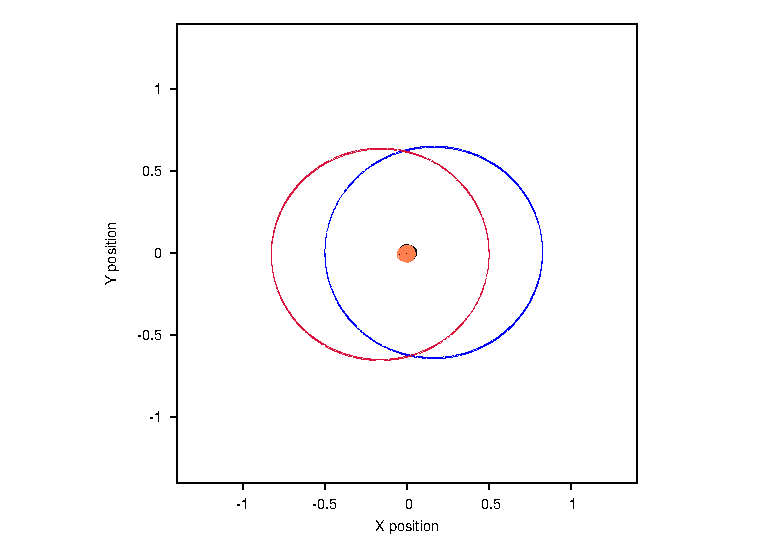
\includegraphics[width=0.9\textwidth]{./2017results/05-75-05-35/Orbit.eps}
\caption{Configuration 17}
\label{fig:config17}
\end{figure}
\begin{figure}[H]
\centering
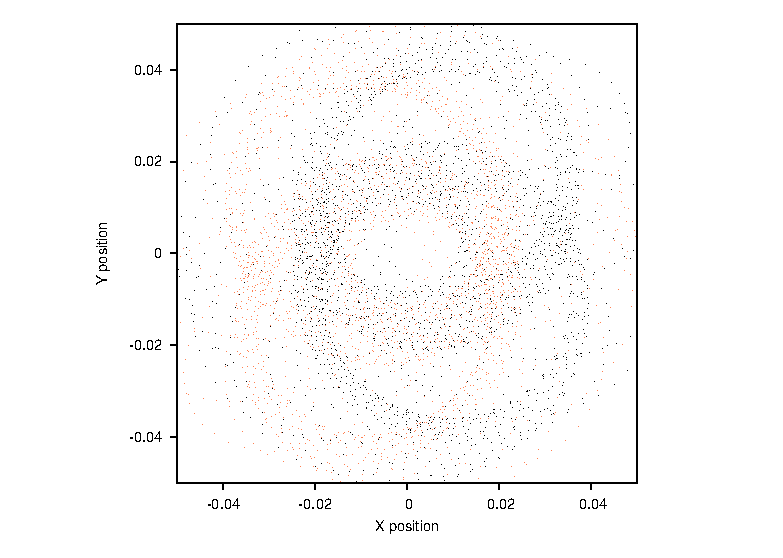
\includegraphics[width=0.9\textwidth]{./2017results/05-75-05-35/Inner.eps}
\caption{Configuration 17 - Inner Bar}
\label{fig:config17i}
\end{figure}

\begin{figure}[H]
\centering
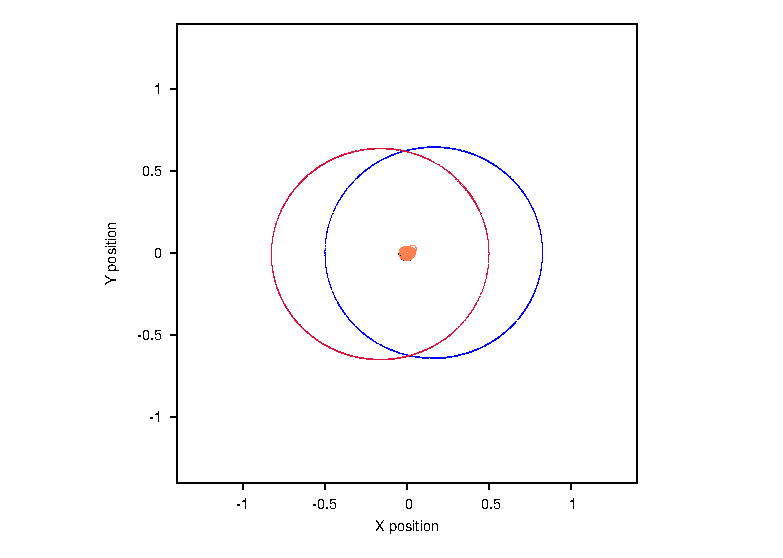
\includegraphics[width=0.9\textwidth]{./2017results/05-75-05-3/Orbit.eps}
\caption{Configuration 18}
\label{fig:config18}
\end{figure}
\begin{figure}[H]
\centering
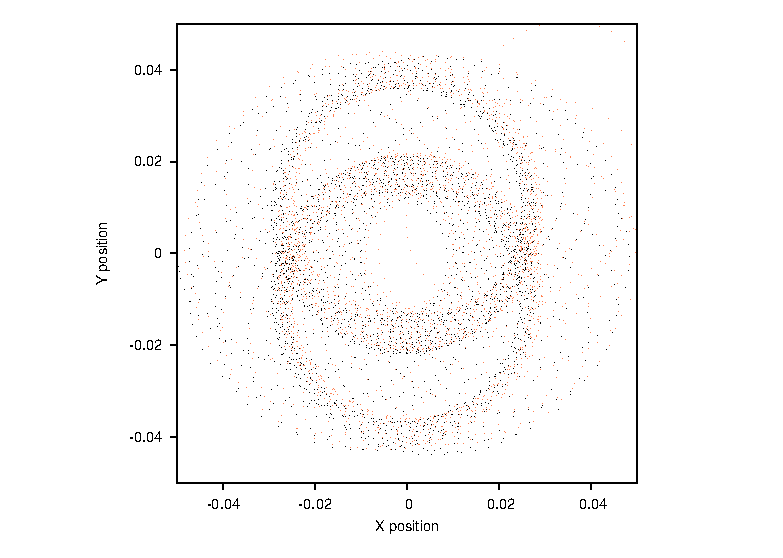
\includegraphics[width=0.9\textwidth]{./2017results/05-75-05-3/Inner.eps}
\caption{Configuration 18 - Inner Bar}
\label{fig:config18i}
\end{figure}

\begin{figure}[H]
\centering
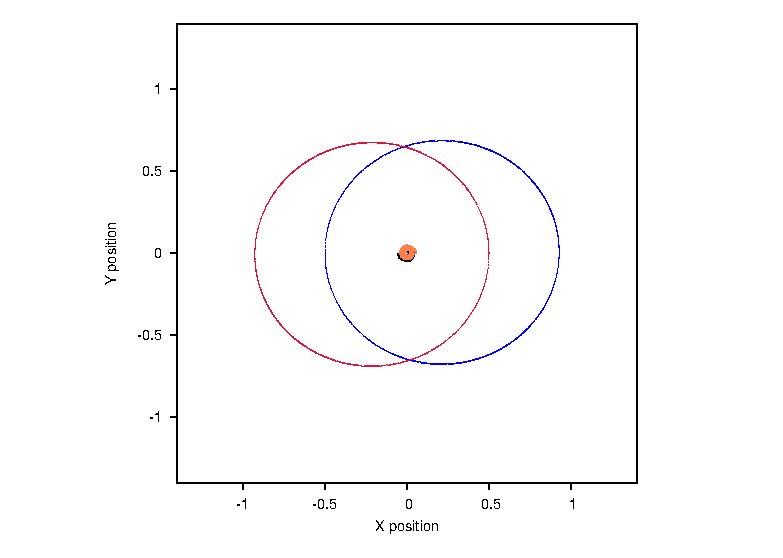
\includegraphics[width=0.9\textwidth]{./2017results/06-8-06-25/Orbit.eps}
\caption{Configuration 19}
\label{fig:config19}
\end{figure}
\begin{figure}[H]
\centering
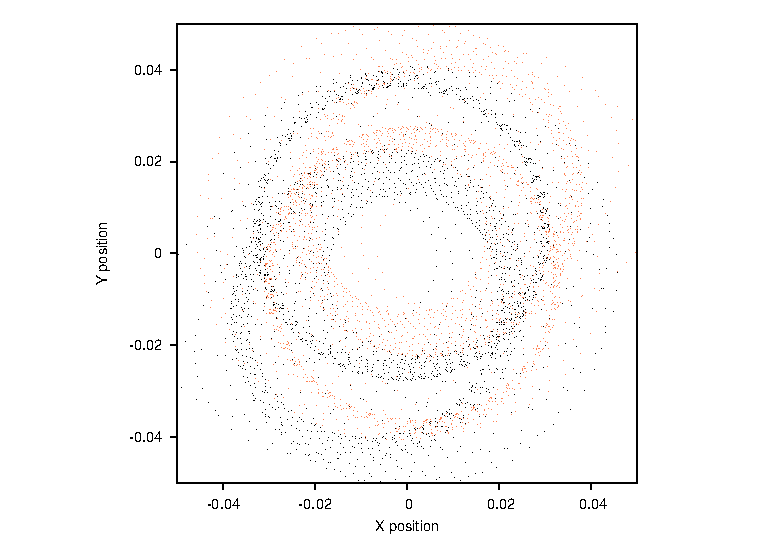
\includegraphics[width=0.9\textwidth]{./2017results/06-8-06-25/Inner.eps}
\caption{Configuration 19 - Inner Bar}
\label{fig:config19i}
\end{figure}

\begin{figure}[H]
\centering
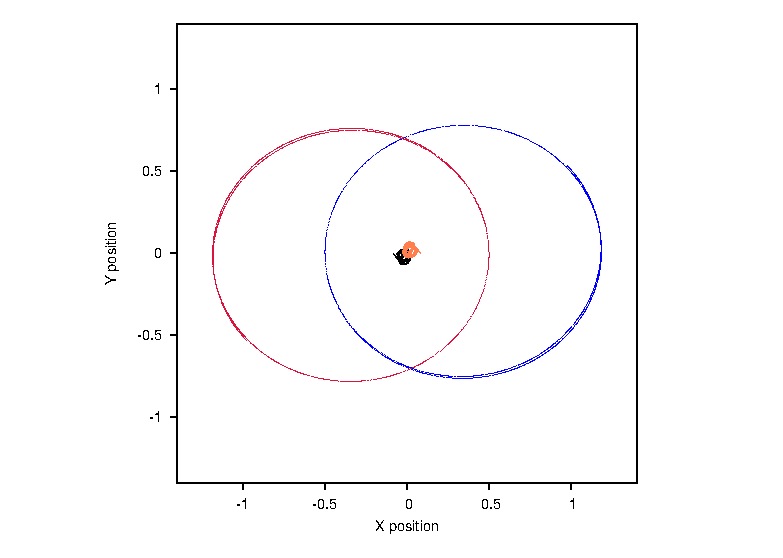
\includegraphics[width=0.9\textwidth]{./2017results/08-9-08-15/Orbit.eps}
\caption{Configuration 20}
\label{fig:config20}
\end{figure}
\begin{figure}[H]
\centering
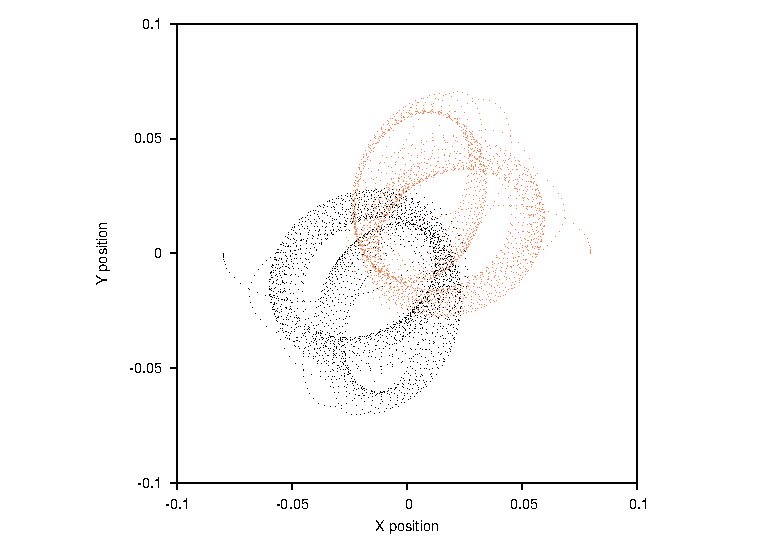
\includegraphics[width=0.9\textwidth]{./2017results/08-9-08-15/Inner.eps}
\caption{Configuration 20 - Inner Bar}
\label{fig:config20i}
\end{figure}

\begin{figure}[H]
\centering
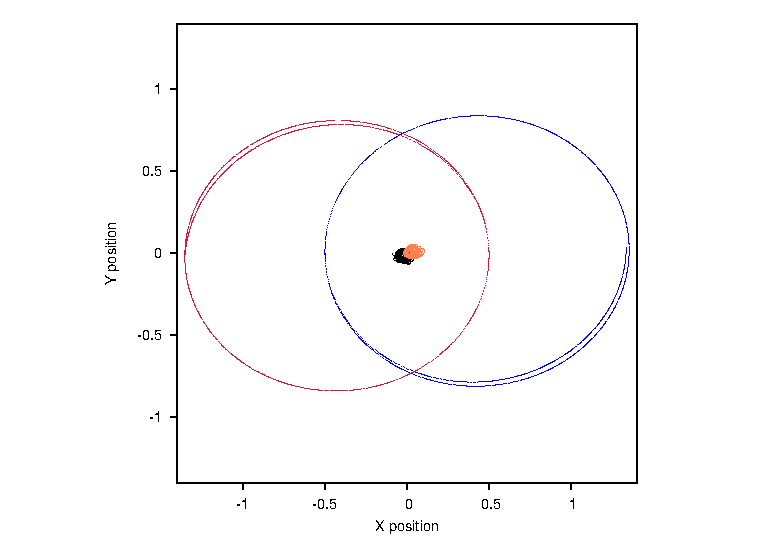
\includegraphics[width=0.9\textwidth]{./2017results/09-95-09-1/Orbit.eps}
\caption{Configuration 21}
\label{fig:config21}
\end{figure}
\begin{figure}[H]
\centering
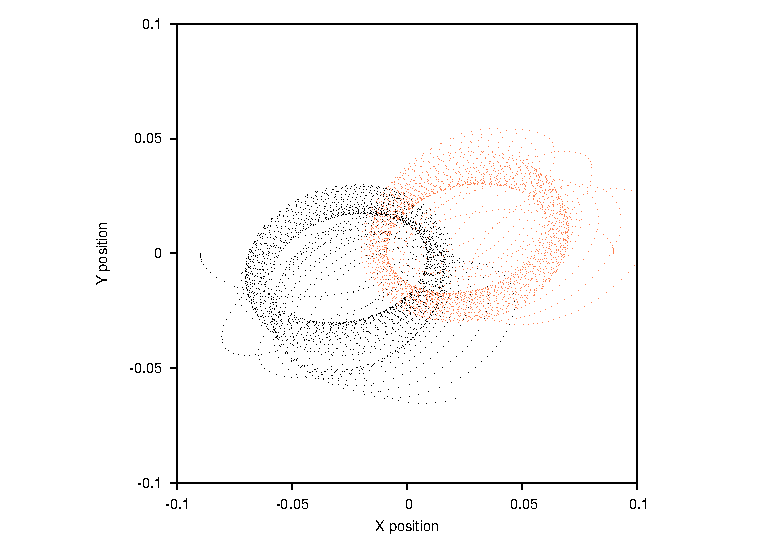
\includegraphics[width=0.9\textwidth]{./2017results/09-95-09-1/Inner.eps}
\caption{Configuration 21 - Inner Bar}
\label{fig:config21i}
\end{figure}

\begin{figure}[H]
\centering
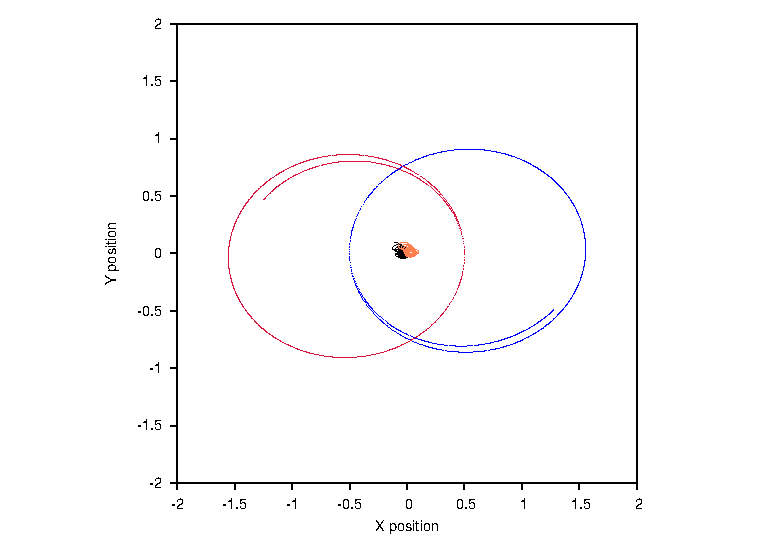
\includegraphics[width=0.9\textwidth]{./2017results/1-1-1-05/Orbit.eps}
\caption{Configuration 22}
\label{fig:config22}
\end{figure}
\begin{figure}[H]
\centering
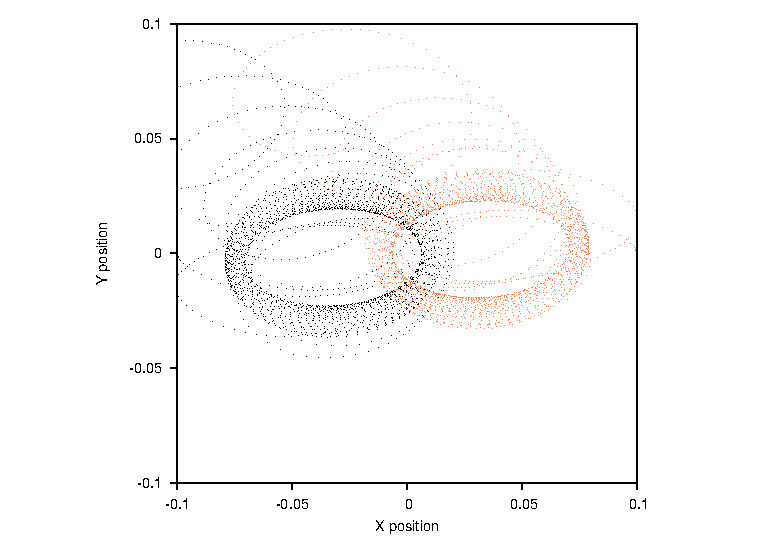
\includegraphics[width=0.9\textwidth]{./2017results/1-1-1-05/Inner.eps}
\caption{Configuration 22 - Inner Bar}
\label{fig:config22i}
\end{figure}

\begin{figure}[H]
\centering
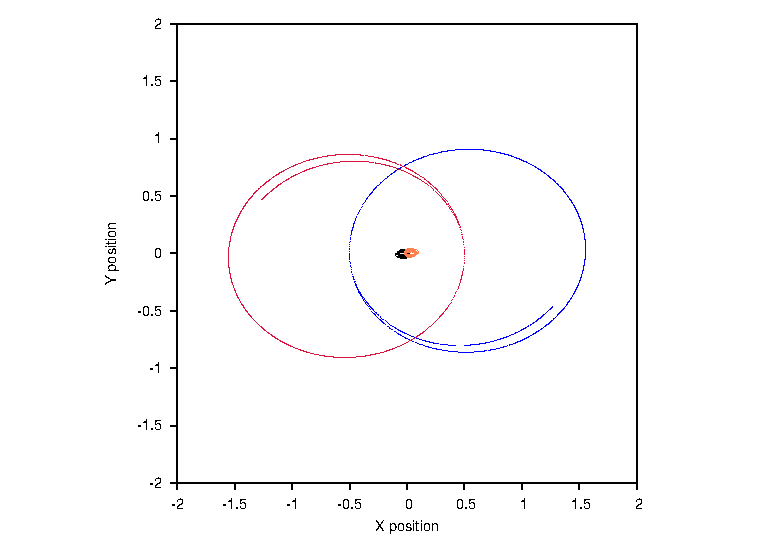
\includegraphics[width=0.9\textwidth]{./2017results/1-1-1-04/Orbit.eps}
\caption{Configuration 23}
\label{fig:config23}
\end{figure}
\begin{figure}[H]
\centering
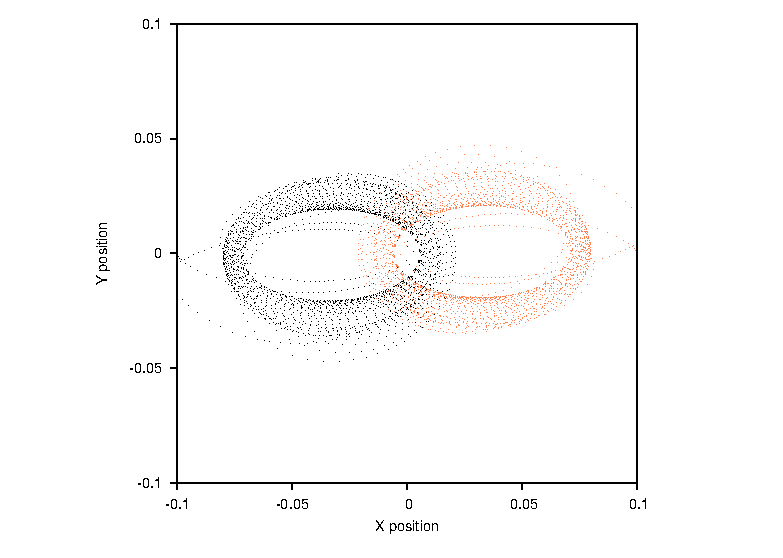
\includegraphics[width=0.9\textwidth]{./2017results/1-1-1-04/Inner.eps}
\caption{Configuration 23 - Inner Bar}
\label{fig:config23i}
\end{figure}

\begin{figure}[H]
\centering
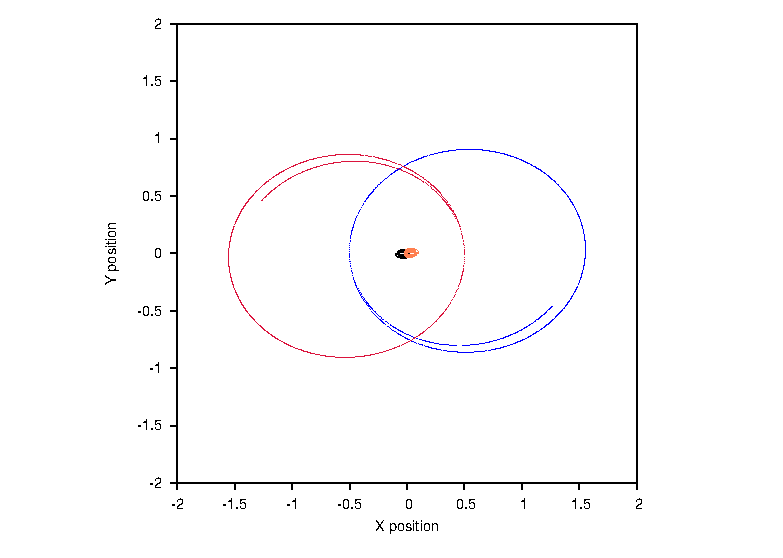
\includegraphics[width=0.9\textwidth]{./2017results/1-1-1-03/Orbit.eps}
\caption{Configuration 24}
\label{fig:config24}
\end{figure}
\begin{figure}[H]
\centering
\includegraphics[width=0.9\textwidth]{./2017results/1-1-1-03/Inner.eps}
\caption{Configuration 24 - Inner Bar}
\label{fig:config24i}
\end{figure}

\begin{figure}[H]
\centering
\includegraphics[width=0.9\textwidth]{./2017results/1-1-1-02/Orbit.eps}
\caption{Configuration 25}
\label{fig:config25}
\end{figure}
\begin{figure}[H]
\centering
\includegraphics[width=0.9\textwidth]{./2017results/1-1-1-02/Inner.eps}
\caption{Configuration 25 - Inner Bar}
\label{fig:config25i}
\end{figure}

\begin{figure}[H]
\centering
\includegraphics[width=0.9\textwidth]{./2017results/12-105-11-015/Orbit.eps}
\caption{Configuration 26}
\label{fig:config26}
\end{figure}
\begin{figure}[H]
\centering
\includegraphics[width=0.9\textwidth]{./2017results/12-105-11-015/Inner.eps}
\caption{Configuration 26 - Inner Bar}
\label{fig:config26i}
\end{figure}

\begin{figure}[H]
\centering
\includegraphics[width=0.9\textwidth]{./2017results/12-11-11-015/Orbit.eps}
\caption{Configuration 27}
\label{fig:config27}
\end{figure}
\begin{figure}[H]
\centering
\includegraphics[width=0.9\textwidth]{./2017results/12-11-11-015/Inner.eps}
\caption{Configuration 27 - Inner Bar}
\label{fig:config27i}
\end{figure}

\begin{figure}[H]
\centering
\includegraphics[width=0.9\textwidth]{./2017results/12-11-115-015/Orbit.eps}
\caption{Configuration 28}
\label{fig:config28}
\end{figure}
\begin{figure}[H]
\centering
\includegraphics[width=0.9\textwidth]{./2017results/12-11-115-015/Inner.eps}
\caption{Configuration 28 - Inner Bar}
\label{fig:config28i}
\end{figure}

\begin{figure}[H]
\centering
\includegraphics[width=0.9\textwidth]{./2017results/12-11-12-015/Orbit.eps}
\caption{Configuration 29}
\label{fig:config29}
\end{figure}
\begin{figure}[H]
\centering
\includegraphics[width=0.9\textwidth]{./2017results/12-11-12-015/Inner.eps}
\caption{Configuration 29 - Inner Bar}
\label{fig:config29i}
\end{figure}

\begin{figure}[H]
\centering
\includegraphics[width=0.9\textwidth]{./2017results/1-1-1-1/Orbit.eps}
\caption{Configuration 30}
\label{fig:config30}
\end{figure}
\begin{figure}[H]
\centering
\includegraphics[width=0.9\textwidth]{./2017results/1-1-1-1/Inner.eps}
\caption{Configuration 30 - Inner Bar}
\label{fig:config30i}
\end{figure}

\begin{figure}[H]
\centering
\includegraphics[width=0.9\textwidth]{./2017results/1-1-102-1/Orbit.eps}
\caption{Configuration 31}
\label{fig:config31}
\end{figure}
\begin{figure}[H]
\centering
\includegraphics[width=0.9\textwidth]{./2017results/1-1-102-1/Inner.eps}
\caption{Configuration 31 - Inner Bar}
\label{fig:config31i}
\end{figure}

\begin{figure}[H]
\centering
\includegraphics[width=0.9\textwidth]{./2017results/1-1-1021-1/Orbit.eps}
\caption{Configuration 32}
\label{fig:config32}
\end{figure}
\begin{figure}[H]
\centering
\includegraphics[width=0.9\textwidth]{./2017results/1-1-1021-1/Inner.eps}
\caption{Configuration 32 - Inner Bar}
\label{fig:config32i}
\end{figure}

\newpage
\section{Disussion}
The final three runs (configurations 30, 31, and 32) were by far the most stable. The orbital periods vary slightly with time so it is difficult to give accurate figures, so
I am using the periods of the first orbit. The following table shows the periods of the two binaries together with the ratios of the corresponding periods.
\begin{table}[ht!]
  \centering
  \caption{Periods}
  \label{tab:periods}
  \begin{tabular}{ccccc}
   Config. & Inner & Outer & Ratio & Length of simulation\\
    \hline
   30 & .51 & 11.56 & 1:22.7 & 25\\
   31 & .54 & 11.5 & 1:21.3 & 25\\
   32 & .55 & 11.5 & 1:20.9 & 35\\
  \end{tabular}
\end{table}
The data shows that as the periodic ratios tends towards 1:21 the system considerably stabilises. Run 32 was by far the most stable run and the orbits persisted until the integrator
errored with a 'Step size underflow'. 1:21 could possibly be an orbital resonance.
Fourier analysis?
Rewrite in Python, automate, introduce machine laerning algoriythm 

\citep{garzon}, \citep{erwin1}, \citep{macie1}, \citep{macie2}, \citep{macie3}, \citep{macie4}, \citep{macie5}
\citep{macie6}, \citep{macie7}, \citep{manos}, \citep{shen1}, \citep{shen2}, \citep{debattista}, \citep{malhotra}

\newpage
\begin{thebibliography}{1}
\bibitem[Aarseth(2003)]{aarseth}Aarseth, S., Gravitational N-Body Simulations, 2003, Cambridge University Press
\bibitem[Alvarez–Ramirez and Medina(2014)]{alvarez}Alvarez–Ramirez, M., Medina, M., A Review of the Planar Caledonian Four-Body Problem, 2014
\bibitem[Binney and Tremaine(2008)]{binney}Binney, J., Tremaine, S., Galactic Dynamics, 2008, Princeton University Press
%\bibitem[Collins(2004)]{collins}Collins, G., The Foundations Of Celestial Mechanics, 2004, Pachart Publishing House
\bibitem[de Vaucouleurs(1975)]{vaucouleurs}de Vaucouleurs, G., 1975, ApJS,29, 193
\bibitem[Debattista and Shen(2007)]{debattista}Debattista, V., Shen, J., Long-Lived Double-Barred Galaxies from Psuedobulges, 2007, The Astrophysical Journal, 654: L127–L130, 2007 January 10
\bibitem[Du et. al.(2015)]{du1}Du, M., Shen, J., Debattista, V., Forming Double-Barred Galaxies from Dynamically Cool Inner Disks, 2015, The Astrophysical Journal, 804:139 (10pp), 2015 May 10 
%\bibitem[Du et. al.(2016)]{du2}Du, M., Debattista, V., Shen, J., Kimematic Properties of Double-Barred Galaxies: Simulations vs. Integral-Field Observations, 2016, arXiv:1607.00585v1
\bibitem[Erwin(2003)]{erwin3}Erwin, P., Double-Barred Galaxies I. A Catalog of Barred Galaxies with Stellar Secondary Bars and Inner Disks, 2003, arXiv:astro-ph/0310806v2
\bibitem[Erwin(2011)]{erwin2}Erwin, P., Double-Barred Galaxies, 2011, Mem. S.A.It. Suppl. Vol. 18, 145
\bibitem[Erwin and Sparke(2002)]{erwin1}Erwin, P., Sparke, L., Double Bars, Inner Disks, and Nuclear Rings in Early-Type Disk Galaxies, 2002, The Astronomical Journal, 124:65–77, 2002 July
\bibitem[Garzon(2014)]{garzon}Garzon, F., Lopez-Corredoira, M., Dynamical evolution of two associated galactic bars, 2014, arXiv:1409.1916.v1
\bibitem[Heggie and Hut(2003)]{heggie}Heggie D., Hut, P., The Gravitational Million-Body Problem, 2003, Cambridge University Press
\bibitem[Lorenzo-Caceres et. al.(2002)]{lorenzo1}de Lorenzo-Caceres, A., Vazdekis, A., Aguerri, K., A., L., Corsini, E., M., Debattista, V., P., Constraining the formation of inner bars. Photometry, kinematics and stellar populations in NGC357⋆, 2002, arXiv:1111.1718v1
\bibitem[Lorenzo-Caceres et. al.(2013)]{lorenzo2}de Lorenzo-Caceres, A., Falcon-Barroso, J., Vazdekis, A., Distinct stellar populations in the inner bars of double-barred galaxies, 2013, arXiv:1302.5701v1
\bibitem[Maciejewski et. al.(2001)]{macie8}Maciejewski, W., Teuben, P., J., Sparke, L., S., Stone, J., M., Gas Inflow in Barred Galaxies - Effects of Secondary Bars, arXiv:astro-ph/0109431v1
%\bibitem[Maciejewski(2002)]{macie1}Maciejewski, W., Constraints on nested bars – implications for gas inflow, 2002, arXiv:astro-ph/0202110v1
%\bibitem[Maciejewski(2003)]{macie2}Maciejewski, W., Chaos or Order in Double Barred Galaxies?, 2003, arXiv:astro-ph/0304432v1
\bibitem[Maciejewski(2008)]{macie3}Maciejewski, W., Orbits in corotating and counterrotating double bars, 2008, arXiv:0801.1471v1
%\bibitem[Maciejewski and Athanassoula(2008)]{macie4}Maciejewski, W., Athanassoula, A., Regular motions in double bars. II. Survey of trajectories and 23 models, 2008, arXiv:0805.3967v1
\bibitem[Maciejewski and Small(2010)]{macie5}Maciejewski, W., Small, E., Orbital Support of Fast and Slow Inner Bars in Double Barred Galaxies, 2010, arXiv:1006.4574v1
\bibitem[Maciejewski and Sparke(1998)]{macie6}Maciejewski, W., Sparke, L., Bars within Bars in Galaxies, 1998, arXiv:astro-ph/9812228v1
\bibitem[Maciejewski and Sparke(1999)]{macie7}Maciejewski, W., Sparke, L., Orbits Supporting Bars within Bars, 1999, arXiv:astro-ph/9911281v1
\bibitem[Malhotra(1998)]{malhotra}Malhotra, R., Orbital Resonances and Chaos in the Solar System, 1998, Solar system Formation and Evolution ASP Conference Series, Vol. 149, 1998
\bibitem[Manos and Athanassoula(2011)]{manos}Manos, T., Athanassoula, E., Regular and chaotic orbits in barred galaxies - I. Applying the SALI/GALI method to explore their distribution in several models, 2011, arXiv:1102.1157v2
\bibitem[Moiseev(2001)]{moiseev}Moiseev, A., V., Velocity dispersion of stars and gas motion in double-barred galaxies, 2001, arXiv:astro-ph/0111220v1
%\bibitem[Moulton(1914)]{moulton}Moulton, F., An Introduction to Celestial Mechanics, 1914, Palmyrin Library 
\bibitem[Press et. al.(1992)]{press}Press, W., H., Teukolsky, S., A., Vetterling, W., T., Flannery, B., P., Numerical Recipes in Fortran 77 The Art of Scientific Computing, 2nd edition
\bibitem[Saha and Maciejewski(2013)]{saha}Saha, K., Maciejewski, W., Spontaneous formation of double bars in dark matter dominated galaxies, 2013, arXiv:1304.7108v1
\bibitem[Sellwood and Wilkinson(2006)]{sellwood}Sellwood, J., Wilkinson, A., Dynamics of Barred Galaxies, 2006, arXiv:astro-ph/0608665v1
\bibitem[Shen and Debattista(2008)]{shen1}Shen, J., Debattista, V., Long-lived double-barred galaxies in N-body simulations, 2008, Mem. S.A.It. Vol. 00, 169
\bibitem[Shen and Debattista(2009)]{shen2}Shen, J., Debattista, V., Observable Properties of Double-Barred Galaxies in N-Body Simulations, 2009, The Astrophysical Journal, 690:758–772, 2009 January 1
\bibitem[Shlosman et. al.(1989)]{shlosman}Shlosman, I., Frank, J., Begeman, M.,C., 1989, Nature, 338, 45
\bibitem[Steves and Roy(1998)]{steves}Steves, B., Roy, A., Some special restricted four-body problems-I. Modelling the Caledonian problem, 1998, Phrt. Spucx, Si., Vol. 46. No. I I /) 12, pp. 1465-1474, 1998
\bibitem[Szell et. al.(2004)]{szell}Szell, A., Erdi, B., Sandor, Zs., Steves, B., Chaotic and stable behaviour in the Caledonian Symmetric Four-Body Problem, 2004, Mon. Not. R. Astron. Soc. 347, 380Ð388 (2004)
\bibitem[Trenti and Hut(2008)]{trenti}Trenti, M., Hut, P., Gravitational N-body Simulations, 2008, arXiv:0806.3950v1
\bibitem[Wozniak(2015)]{wozniak}Wozniak, H., How can double-barred galaxies be long-lived?, 2015, A and A 575, A7 (2015)
\end{thebibliography}
\end{document}